%% 该模板修改自《计算机学报》latex 模板
%% 主要是将双栏改成单栏，去掉了部分计算机学报标识；
%% 源文件自：https://www.overleaf.com/latex/templates/latextemplet-cjc-xelatex/ybmmymncrrmw
%% 
%%
%% This is file `CjC_template_tex.tex',
%% is modified by Zhi Wang (zhiwang@ieee.org) based on the template 
%% provided by Chinese Journal of Computers (http://cjc.ict.ac.cn/).
%%
%% This version is capable with Overleaf (XeLaTeX).
%%
%% Update date: 2023/03/10
%% -------------------------------------------------------------------
%% Copyright (C) 2016--2023 
%% -------------------------------------------------------------------
%% This file may be distributed and/or modified under the
%% conditions of the LaTeX Project Public License, either version 1.3c
%% of this license or (at your option) any later version.
%% The latest version of this license is in
%%    https://www.latex-project.org/lppl.txt
%% and version 1.3c or later is part of all distributions of LaTeX
%% version 2008 or later.
%% -------------------------------------------------------------------

\documentclass[10.5pt,compsoc,UTF8]{CjC}
\usepackage{bm}   % 给数学符号加粗
\usepackage{xeCJK}
\setCJKmainfont{STSong}[AutoFakeBold,AutoFakeSlant]
\setCJKsansfont{STHeiti}[AutoFakeBold,AutoFakeSlant]
\setCJKmonofont{STFangsong}
\newcommand{\heiti}{\CJKfamily{STHeiti}}
\newcommand{\songti}{\CJKfamily{STSong}}
\newcommand{\fangsong}{\CJKfamily{STFangsong}}
\newcommand{\kaishu}{\CJKfamily{STKaiti}}
\newcommand{\chinese}[1]{%
  \ifnum\value{#1}=1 一\else
  \ifnum\value{#1}=2 二\else
  \ifnum\value{#1}=3 三\else
  \ifnum\value{#1}=4 四\else
  \ifnum\value{#1}=5 五\else
  \ifnum\value{#1}=6 六\else
  \ifnum\value{#1}=7 七\else
  \ifnum\value{#1}=8 八\else
  \ifnum\value{#1}=9 九\else
  \ifnum\value{#1}=10 十\else
  \ifnum\value{#1}=11 十一\else
  \ifnum\value{#1}=12 十二\else
  \arabic{#1}\fi\fi\fi\fi\fi\fi\fi\fi\fi\fi\fi\fi}
\usepackage{graphicx}
\usepackage{footmisc}
\usepackage{enumitem}
%\usepackage{subfigure}
\usepackage{subcaption}    % 子图/子表
\usepackage{url}
\usepackage{multirow}
\usepackage{multicol}
\usepackage[noadjust]{cite}
\usepackage{amsmath,amsthm}
\usepackage{siunitx}
\usepackage{amssymb,amsfonts}
\usepackage{booktabs}
\usepackage{color}
\usepackage{ccaption}
\usepackage{booktabs}
\usepackage{float}
\usepackage{fancyhdr}
\usepackage{caption}
\usepackage{xcolor,stfloats}
\usepackage{comment}
\setcounter{page}{1}
\graphicspath{{figures/}}
\usepackage{cuted}%flushend,
\usepackage{captionhack}
\usepackage{epstopdf}
\usepackage{gbt7714}
\usepackage{braket}
\usepackage{algorithm}
\usepackage{algpseudocode}
% \usepackage{tikz}
% \usetikzlibrary{quantikz}
\usepackage{amsmath}

% 必须先加载 Xy-pic
\usepackage[all]{xy}

% 然后手动启用 matrix 模块（关键！）
\xyoption{matrix}
\usepackage{qcircuit}
%===============================%

\headevenname{\mbox{\quad}  \hfill  \mbox{\zihao{-5}{ \hfill \hfill 《针对稀疏量子态制备的最优线路研究》  } \hspace {37mm} \mbox{2025 年 8 月}}}%
\headoddname{ \hfill 《针对稀疏量子态制备的最优线路研究》}%

%footnote use of *
\renewcommand{\thefootnote}{\fnsymbol{footnote}}
\setcounter{footnote}{0}
\renewcommand\footnotelayout{\zihao{5-}}

\newtheoremstyle{mystyle}{0pt}{0pt}{\normalfont}{1em}{\bf}{}{1em}{}
\theoremstyle{mystyle}
\renewcommand\figurename{figure~}

%\renewcommand{\thesubfigure}{(\alph{subfigure})}


\newcommand{\upcite}[1]{\textsuperscript{\cite{#1}}}
\renewcommand{\labelenumi}{(\arabic{enumi})}
\newcommand{\tabincell}[2]{\begin{tabular}{@{}#1@{}}#2\end{tabular}}
\newcommand{\abc}{\color{white}\vrule width 2pt}
\renewcommand{\bibsection}{}
\makeatletter
\renewcommand{\@biblabel}[1]{[#1]\hfill}
\makeatother
\setlength\parindent{2em}
%\renewcommand{\hth}{\begin{CJK*}{UTF8}{gbsn}}
%\renewcommand{\htss}{\begin{CJK*}{UTF8}{gbsn}}


\DeclareCaptionLabelFormat{chinese}{#1~\chinese{figure}}
\captionsetup[figure]{
  labelformat = simple,
  labelsep = quad,
  name = 图,
  font = bf % 这里添加 font = bf 使图号加粗
}



\renewcommand{\thefigure}{\chinese{figure}}




\begin{document}

\hyphenpenalty=50000
\makeatletter
\newcommand\mysmall{\@setfontsize\mysmall{7}{9.5}}
\newenvironment{tablehere}
  {\def\@captype{table}}

\let\temp\footnote
\renewcommand \footnote[1]{\temp{\zihao{-5}#1}}


\thispagestyle{plain}%
\thispagestyle{empty}%
\pagestyle{CjCheadings}

% \begin{table*}[!t]
\vspace {-13mm}


\onecolumn
\zihao{5-}\noindent \hfill \hspace {11mm} 《针对稀疏量子态制备的最优线路研究》\hfill 2025 年 8 月\\
\noindent\rule[0.25\baselineskip]{\textwidth}{1pt}

% \onecolumn
% \zihao{5-}\noindent 第??卷\quad 第?期 \hfill 计\quad 算\quad 机\quad 学\quad 报\hfill Vol. ??  No. ?\\
% \zihao{5-}
% 20??年?月 \hfill CHINESE JOURNAL OF COMPUTERS \hfill ???. 20??\\ 
% \noindent\rule[0.25\baselineskip]{\textwidth}{1pt}

{
\centering
\vspace {11mm}
{\zihao{2} \heiti 针对稀疏量子态制备的最优线路研究 }

\vskip 5mm

% {\zihao{4}\fangsong 作者名$^{1)}$\quad  作者名$^{2),3)}$ \quad 作者名$^{3) }$($^*$字体为3号仿宋*作者)}

% \footnote{\noindent \zihao{6} 
% % 收稿日期：\quad \quad -\quad -\quad ；最终修改稿收到日期：\quad \quad -\quad -\quad .*投稿时不填写此项*. 本课题得到… …基金中文完整名称(No.项目号)、… …基金中文完整名称(No.项目号)、… … 基金中文完整名称(No.项目号)资助.
% \textsf{作者名1}，学号，学位(或目前学历),主要研究领域为*****、****. E-mail: **************.\textsf{作者名2}，学号，学位(或目前学历),主要研究领域为*****、****. E-mail: **************. \textsf{作者名3}，学号，学位(或目前学历),主要研究领域为*****、****. E-mail: **************.}

% \vspace {5mm}

% \zihao{5}{$^{1)}$(单位全名 部门(系)全名, 市(或直辖市) 国家名 邮政编码) *字体为5号宋体*单位}

% \zihao{5}{$^{2)}$(单位全名 部门(系)全名, 市(或直辖市) 国家名 邮政编码)*中英文单位名称、作者姓名须一致*}

% \zihao{5}{$^{3)}$(单位全名 部门(系)全名, 市(或直辖市) 国家名 邮政编码)}

% \zihao{6}{\textsf{论文定稿后，作者署名、单位无特殊情况不能变更。若变更，须提交签章申请，国家为中国可以不写，省会城市不写省名，其他国家必须写国家名。}}
}

\vskip 5mm

\zihao{5}{
\setlength{\baselineskip}{16pt}\selectfont{
\noindent {\heiti 摘\quad 要\quad }

量子态制备问题是量子计算的基本问题，也是量子线路编译的关键部分。在一般量子态制备的算法中，生成的线路规模会随着量子比特数量呈指数增长。然而，许多实际相关的状态在标准基中较为稀疏，这种稀疏性在态制备问题中有着天然的优势。基于此，我们提出了一种多项式时间算法，该算法能够在不使用辅助比特的情况下针对给定的稀疏态设计对应的实现线路进行精确制备。我们数值验证了当非零相位数量等于比特数量时，相比于目前最优的稀疏态制备算法，当比特数量为$10$时，我们算法可以节省$19.73\%$的线路长度；当比特数量为$15$时，我们算法可以节省$22.28\%$的线路长度；当比特数量为$50$时，我们算法可以节省$16.86\%$的线路长度。考虑NISQ设备的特定结构，我们通过增加线路局部性将原始全连接电路在保持逻辑等价的前提下优先重写为近邻交互，将电路高效映射到Heavy-Hex与Square等非全连接耦合图上，与目前最优方法相比，当量子比特数量为10时，Heavy-Hex拓扑结构可以节约19.70\%的线路长度，Square\_25可以节约26.18\%的线路长度，最高可以节约37.60\%的线路长度。同时，我们设计一个软件包，改软件包好上手，可以促进使用人员的算法探索，也便于没有量子线路基础的研究人员使用该算法。


\par}}
\vspace {5mm}

\zihao{5}{\noindent
{\heiti 关键词 \quad }{量子计算；量子线路优化；量子态制备； 稀疏态制备； 多控Toffoli门}
}
% \zihao{5-}{\heiti 中图法分类号\quad } TP\rm{\quad \quad \quad     }
% {\heiti DOI号:\quad } *投稿时不提供DOI号


% \vskip 7mm

% \begin{center}
% \zihao{3}{ \heiti Title *（中英文题目一致)字体为4号Times New Roman,加粗* Title}\\
% \vspace {5mm}
% \zihao{5}{ NAME Name-Name$^{1)}$ NAME Name$^{2)}$ NAME Name-Name$^{3)}$ *字体为5号Times new Roman*Name}\\
% \vspace {2mm}
% \zihao{5-}{{$^{1)}$(Department of ****, University, City ZipCode, China) *字体为小5号Times new Roman* Depart.Correspond}}

% \zihao{5-}{{$^{2)}$(Department of ****, University, City ZipCode)*中国不写国家名*}}

% \zihao{5-}{{$^{3)}$(Department of ****, University, City ZipCode, country)*外国写国家名*}}

% \end{center}

% \zihao{5}{
% \setlength{\baselineskip}{18pt}\selectfont{
% {\bf Abstract}\quad (\textbf{500英文单词，内容包含中文摘要的内容}).
% 字体为Times new Roman,字号5号* 
% \zihao{5}{\noindent Do not modify the amount of space before and after the artworks. One- or two-column format artworks are preferred. and Tables, create a new break line and paste the resized artworks where desired. Do not modify the amount of space before and after the artworks. One- or two-column format artworks are preferred. All Schemes, Equations, Figures, and Tables should be mentioned in the text consecutively and numbered with Arabic numerals, and appear below where they are mentioned for the first time in the main text. To insert Schemes, Equations, Figures, and Tables, create a new break line and paste the resized artworks where desired. Do not modify the amount of space before and after the artworks. One- or two-column format artworks are preferred.Do not modify the amount of space before and after the artworks. One- or two-column format artworks are preferred. and Tables, create a new break line and paste the resized artworks where desired. %Do not modify the amount of space before and after the artworks. One- or two-column format artworks are preferred. All Schemes, Equations, Figures, and Tables should be mentioned in the text consecutively and numbered with Arabic numerals, and appear below where they are mentioned for the first time in the main text.
% \par}}
% \vspace {5mm}

% {{\bf Keywords}\quad 中文关键字与英文关键字对应且一致，\textbf{不要用英文缩写});
% key word; key word; key word* *字体为5号Times new Roman * Key words\par}}



%%%%%%%%%%%%%%%%%%%%%%%%%%%%%%%%%%%%%%
\zihao{5}
\vskip 10mm
% \begin{multicols}{1}


%%%%%%%%%%%%%%%%%%%%%%%%%%%%%%%%%%%%%%%%%%
%%%%%%%%%%%%%%%%%%%%%%%%%%%%%%%%%%%%%%%%%%


\section{\heiti 引言}


量子计算自提出以来就表现出解决经典难解问题的强大潜力，其中一些著名的算法有区分平衡函数和常函数的DJ算法\cite{deutsch1992rapid}、量子无序搜索算法\cite{grover1996fast}、量子大整数分解算法\cite{Shor1994Polynominal}等。此外近些年，量子机器学习\cite{biamonte2017quantum}、量子哈密顿量模拟由于其相对经典算法的优越性\cite{berry2015simulating,low2017optimal,low2019hamiltonian,berry2015hamiltonian}都得到了广泛的研究和讨论。量子计算俨然已成为各个国家科研的新动力新方向，在2024年3月展开的十四届人大第二次会议上李强总理也提到``要开展量子技术新赛道''。

在这个NISQ时期，量子编译俨然成为了连通量子算法与量子设备的桥梁，能够将量子算法在量子设备上部署实现。而在量子编译中有一个关键的问题是量子态制备问题，即创建特定初始量子态以编码输入数据或问题实例的过程。量子态的制备对于现有量子算法的实现起着关键作用。通常，量子算法工作的起点就是将通用经典数据编码为量子态。然而，由于叠加态和纠缠态的特殊现象，量子编译过程的某些环节与经典计算中的对应任务存在显著差异，无法直接进行数据迁移。这就会造成量子态制备这一问题往往会产生较大的线路开销。

作为量子计算、量子线路编译的重要部分，量子态制备的复杂度远超经典计算的模拟过程\cite{aaronson2004multilinear}。在经典计算中，通过设置$O\left ( n \right ) $个量子门即可获得$O\left ( n \right ) $大小存储单元的所有可能状态；而量子计算机的状态是基态的叠加态，其中部分状态只能通过极其复杂的电路才能实现\cite{knill1995approximation, mottonen2004transformation} 。事实上，研究表明，仅使用单量子比特门和$CNOT$门的门库时，$n$量子比特量子计算机的一般量子态制备只能通过规模为$\Omega \left ( 2^n \right ) $\cite{knill1995approximation, mottonen2004transformation} 的线路来制备。由于一般量子态制备的线路成本较高，且实际应用中往往呈现特殊结构，已经存在针对振幅由连续函数给出的状态、通过黑盒预言机获取振幅的状态等特殊量子态\cite{bausch2022fast, gonzalez2024efficient, holmes2020efficient, marin2023quantum, rattew2022preparing, sanders2019black}制备的研究成果。

然而，与一般态不同的是，现实中大多数的量子态都是只有极少数基态具有非零系数，我们将这类具有该特性的态称为稀疏量子态。并且出现了许多针对稀疏量子态制备的相关研究。在不使用辅助比特的情况下，Gidney等\cite{gleinig2021efficient, malvetti2021quantum}提出的方法以$O\left ( \left |  S\right | n \right ) $的线路复杂度实现稀疏态制备，随后Li\cite{li2024nearly}又改进到$O\left (  \frac{\left |  S\right | n}{\log_{}{n} } + n\right) $。在使用两个辅助比特的情况下Mao\cite{mao2024toward}提出的方法使用$O\left (  \frac{\left |  S\right | n}{\log_{}{n} } \right) $的线路复杂度实现稀疏态制备。然而，针对实际制备的线路数值进行比较，Gidney\cite{gleinig2021efficient}提出的相位缩减方法仍为目前最优方法。

基于此，本文针对稀疏量子态制备的线路长度进行研究，提出了一种多项式时间算法。与先前工作不同的是，本文以实际应用为出发，研究线路长度的实际数值优化。与目前数值最优的稀疏态制备方法\cite{gleinig2021efficient}相比，本文算法在比特数量和量子非零相位数量都为$10$时，我们算法可以节省$19.73\%$的$CNOT$门；当比特数量和量子非零相位数量都为$15$时，我们算法可以节省$22.28\%$的$CNOT$门。并且随着非零相位数量的增加，我们的算法会表现出更大的优势。当在比特数量为$10$非零相位数量为$50$时,我们算法可以节省$25.54\%$的$CNOT$门。

本文结构如下，第二节介绍准备工作，第三节介绍我们的方法，第四节介绍基于AI引导的平行多面体搜索优化策略，第五节为数值实验评估和我们的工具包，第六章为结论和未来展望。值得注意的是，我们给出了一个稀疏态制备的案例，和我们软件包的使用方法。


%%%%%%%%%%%%%%%%%%%%%%%%%%%%%%%%%%%%%%%%%%
%%%%%%%%%%%%%%%%%%%%%%%%%%%%%%%%%%%%%%%%%%


\section{\heiti 准备工作}
\subsection{\heiti 稀疏量子态}
在包含 $n$ 个量子比特的系统中，计算基态共有 $2^{n}$ 个相互正交的向量$\ket{00\dots00},\; \ket{00\dots01},\; \dots,\; \ket{11\dots11}$, 分别对应长度为 $n$ 的二进制串。任意量子态 $\ket{\psi}$ 可写成这些基态的归一化线性组合：
\begin{equation}
\ket{\psi} = \sum_{c\in\{0,1\}^{n}}\alpha_{c}\ket{c},\qquad
\sum_{c\in\{0,1\}^{n}}|\alpha_{c}|^{2}=1
\end{equation}
\par
其中 $\alpha_{c}$ 称为振幅。若绝大多数 $\alpha_{c}=0$，仅少量非零，则称该态为\textit{稀疏量子态}。
记非零振幅对应的二进制串集合为 $S\subset\{0,1\}^{n}$，则
\begin{equation}
\ket{\psi} = \sum_{c\in S}\alpha_{c}\ket{c}
\end{equation}

当 $|S|\ll 2^{n}$ 时，只需存储集合 $S$ 及其对应的非零振幅 $\alpha_{c}$，即可比完整记录 $2^{n}$ 个系数更高效地描述该量子态。

\subsection{\heiti 量子门与量子线路}


\subsubsection*{\heiti1. 单量子比特门}
对任意单量子比特态 $|\psi\rangle=\alpha|0\rangle+\beta|1\rangle$，单量子比特门由 $2\times 2$ 的酉矩阵 $U$ 实现，满足
$$U^\dagger U = UU^\dagger = I_2,$$
其中 $U^\dagger$ 表示 $U$ 的共轭转置，$I_2$ 为 $2$ 维单位矩阵。
该门作用后的态为$$|\psi'\rangle = U|\psi\rangle
$$一般地，单量子比特门可实现任意 $SU(2)$ 变换。

\subsubsection*{\heiti 2. CNOT 门（受控非门）}
CNOT 门作用于两量子比特，设第一个比特为控制比特，第二个比特为目标比特，其矩阵表示为
\[
\mathrm{CNOT} =
\begin{pmatrix}
1 & 0 & 0 & 0\\
0 & 1 & 0 & 0\\
0 & 0 & 0 & 1\\
0 & 0 & 1 & 0
\end{pmatrix}
\]\par
该门在计算基下的作用为
\[
\mathrm{CNOT}|c\rangle|t\rangle = |c\rangle|c\oplus t\rangle,\quad c,t\in\{0,1\}
\]\par
在本文中，将选取单量子比特门与CNOT门作为基础门进行量子线路构建。


\subsubsection*{\heiti 3. 多控Toffoli 门}

量子线路中的\emph{多控 Toffoli 门}（Multi-controlled Toffoli, 记作 $MCT_k$）是经典可逆逻辑门 $k$–Toffoli 的量子推广。
给定 $(k+1)$ 个量子比特，其中前 $k$ 个为控制位 $\ket{c_1c_2\cdots c_k}$，第 $(k+1)$ 个为目标位 $\ket{t}$，
$MCT_k$ 的作用定义为
\begin{equation}
  \label{eq:MCT-def}
  MCT_k\ket{c_1\cdots c_k}\ket{t}
  = \ket{c_1\cdots c_k}\ket{t \oplus (c_1\!\cdot\!c_2\cdots c_k)}
\end{equation}\par
当且仅当所有控制位均为 $\ket{1}$ 时，目标位受 $X$ 门作用；否则保持不变。

其矩阵形式为 $2^{k+1}\times 2^{k+1}$ 的单位矩阵，仅对角元 $X_{2^{k+1}-2,2^{k+1}-2}=X_{2^{k+1}-1,2^{k+1}-1}=0$，
其余对应位置为 Pauli-$X$ 元素，即
\begin{equation}
  \label{eq:MCT-matrix}
  MCT_k = I^{\otimes (k+1)} - \ket{1\cdots1}\!\bra{1\cdots1}\otimes I
  + \ket{1\cdots1}\!\bra{1\cdots1}\otimes X
\end{equation}

特别地，当 $k=2$ 时，$MCT_2$ 即为标准三比特 Toffoli 门（CCX）。
在计算基下的酉作用亦可简洁地写成
\begin{equation}
  MCT_k\ket{c}\ket{t} = \ket{c}\ket{t \oplus \prod_{i=1}^{k}c_i},
  \quad c_i,t\in\{0,1\}
\end{equation}

后续线路构造以 $MCT_k$ 作为核心门集之一；借助 Gidney\cite{Gidney2015} 的方案，该门集可在 $O(\log |S|)$ 个 CNOT 门内实现。

\subsubsection*{\heiti 4. 多控制G门}


在本文的量子线路构造中，我们需要借助一类特殊的单量子比特门
\begin{equation}
  G(\alpha,\omega)=
  \begin{pmatrix}
    e^{i\alpha}\cos\omega & \sin\omega\\[4pt]
    \sin\omega & -e^{i\alpha}\cos\omega
  \end{pmatrix},
\end{equation}\par
该门作用在基态上满足
$
  G(\alpha,\omega)\bigl(\alpha\ket{0}+\beta\ket{1}\bigr)=e^{i\varphi}\ket{0}
$
其中$G(\alpha,\omega)$ 可被高效地实现为多控门：只需将其分解为两个单量子比特门与一个多控 Toffoli 门,而多控 Toffoli 门又可进一步用线性数量的 CNOT 门实现\cite{barenco1995elementary}。

\subsubsection*{\heiti 5. 量子线路}
量子线路是由量子门通过量子门连接而成的序列。  
若线路由门 $G_1,G_2,\ldots,G_k$ 依次作用，其整体酉矩阵为
$
U_{\text{circuit}} = G_k G_{k-1}\cdots G_1
$
为便于阅读，线路图中允许使用多控操作。但在计算线路长度时，由于现有的多Qubit量子门的保真度较低，我们使用 CNOT 门的数量作为线路长度开销。

\subsection{\heiti 问题表述}
 
给定集合 $S\subset\{0,1\}^n$ 及非零系数 $\{\alpha_c\}_{c\in S}$所定义的量子态
$
\ket{\psi}=\sum_{c\in S}\alpha_c\ket{c}
$
，构造由基础量子门 $G_1,G_2,\dots,G_k$ 组成的线路
$
C=G_k G_{k-1}\cdots G_1
$
使得
\begin{equation}
C\ket{0}^{\otimes n}=\ket{\psi}
\end{equation}\par
并要求尽可能减少门数 $k$。由于基础门可逆，若存在线路 $C'$ 满足 $C'\ket{\psi}=\ket{0}^{\otimes n}$，则取逆线路 $(C')^{-1}$ 即可实现正向制备；故在后文中我们统一描述为“寻找将 $\ket{\psi}$ 映射到 $\ket{0}^{\otimes n}$ 的线路”。

%%%%%%%%%%%%%%%%%%%%%%%%%%%%%%%%%%%%%%%%%%
%%%%%%%%%%%%%%%%%%%%%%%%%%%%%%%%%%%%%%%%%%


\section{\heiti 方法}

本文的核心思路为将 $\ket{\psi}$ 拆分为若干“非零相位缩减”的子问题，通过特定受控操作实现两个非零相位合并，最后迭代执行上述操作，最终把所有非零振幅集中到 $\lvert 0\cdots0\rangle$。因此，降低每一次两个非零相位合并的门开销成为关键。若能恰当的减少实现两非零相位合并所需$G$门的控制位数量，就能显著减少所需门数。后文将围绕这一思路展开：先总体展示合并思路，再通过特定算法体现如何选择控制位、受控位与实现门电路的构建，最后通过对比实验，展示该算法的有效性。总体思路实现如Algorithm 1。

\begin{algorithm}[H]
\caption{稀疏态制备}
\begin{algorithmic}[1]
\State \textbf{Input}:一个 $n$ 量子比特量子态的经典描述 $\phi = \sum_{x \in S} c_x |x\rangle$
\State \textbf{Output}:一个电路 $C$ 使得 $C |0^n\rangle = \phi$。
\State 初始化一个空的量子电路 $C$；
\While{$|S| > 1$}
    \State 使用Algorithm 2确定需合并的非零相位与多控G门的控制位$control\_bit$;
    \State 使用Algorithm 3确定多控G门的受控位$dif$;
    \State 使用Algorithm 4找到一个线路 $\hat{C}$ 先实现的两个非零相位仅在受控位dif位上存在差异，且$control\_bit$位均为1，再进一步实现在量子比特 $dif$ 上应用一个由 $control\_bit$ 中的量子比特控制的 $G$ 门，实现 $\hat{C} \phi = \sum_{x \in S'} c'_x |x\rangle$，其中 $|S'| = |S|-1$
   
    \State 更新状态 $\phi = \hat{C}  \phi$；
    \State 更新电路 $C = \hat{C} \circ C$；
\EndWhile
\State 在 $C$ 中添加将 $\phi$ 转换为 $|0^n\rangle$ 所需的 NOT 门；

\State 反转 $C$ 中的门并颠倒它们的顺序；

\State \textbf{Return}: $C$；

\end{algorithmic}
\end{algorithm}


\subsection{控制位选择与预合并非零相位确立}
根据 Algorithm 1可知，算法的核心步骤之一在于对两个非零相位用控制$G(\alpha,\omega)\bigl(\alpha\ket{0}+\beta\ket{1}\bigr)=e^{i\varphi}\ket{0}$实现合并。在实际操作过程中，存在控制G门操作意外导致其他非零相位的变化，所以选取存在显著区别的$control\_bit$对于实现非零相位合并的意义重大。具体要求为当且仅当预合并非零相位的$control\_bit$全为1且其他非零相位不完全满足该条件时，才允许实现多控G门操作。为实现该要求，我们通过对每一个量子比特进行最大差异化的选择迭代，快速确立控制比特与合并量子态。具体算法实现见Algorithm 2。算法中的一个核心思想是，由于多控G门的开销大，我们利用$CNOT$门进行处理，使得后续的多控G门的控制位减少，这是算法高效的关键所在。


\begin{algorithm}[H]
\caption{多控G门控制比特选择与预合并非零相位确立}
\begin{algorithmic}[1]
\State \textbf{Input:} 0-1 矩阵 $M \in \{0,1\}^{s \times n}$，其每一行对应一个计算基态 $\ket{x_k}$。
\State \textbf{Output:} 控制比特集合 $control\_bit$；满足 $M_{r_1,q}=M_{r_2,q}$ 的两行下标 $r_1,r_2$；已施加的 CNOT 电路 $C$。

% ---------- 步骤一：直接检索目标列 ----------
\For{$j = 1$ \textbf{至} $n$}
    \State $w_j \gets \sum_{k=1}^{s} M_{k,j}$  \Comment{计算第 $j$ 列的汉明重量}
    \If{$w_j = 2$ \textbf{或} $w_j = s-2$}
        \State 选取满足 $M_{r,j}=M_{r',j}$ 的两行 $r_1,r_2$ \Comment{即所选比特值相同}
        \State \Return $(j,\, r_1,\, r_2,\, C = \emptyset)$
    \EndIf
\EndFor

% ---------- 步骤二：迭代施加 CNOT ----------
\State $C \gets \emptyset$  \Comment{初始 CNOT 门序列为空}
\While{True}
\State 接受上次循环输出的新矩阵，若第一次循环则接受原矩阵
\For{$i = 1$ \textbf{至} $n$}
\For{$j = i+1$ \textbf{至} $n$}
\State 设 $w_{i\oplus j}$ 表示列 $i$ 与列 $j$ 逐位异或后的重量
    \State 设$\Delta_{i,j}$表示$i$列与$j$列异或前后，最小重量的差值
    $$
        \Delta_{i,j} = \min(w_i,w_j,s-w_i,s-w_j) - \min(w_{i\oplus j},\, s-w_{i\oplus j})
    $$
    \If{$\Delta_{i,j}>1\text{且}\max(w_i,w_j,s-w_i,s-w_j)=\max(w_i,s-w_i)$}
    \State 将 $\textsc{cnot}(i,j)$ 追加到 $C$，表示$i$为受控位，$j$为控制位并更新第 $j$ 列：
    \[
        M_{k,i} \gets M_{k,i} \oplus M_{k,j}, \quad \forall k \in [1..s]
    \]
    \ElsIf{$\Delta_{i,j}>1\text{且}\max(w_i,w_j,s-w_i,s-w_j)=\max(w_j,s-w_j)$}
    \State 重复第一个判断操作，但是替换$i,j$的位置
    \EndIf
    \If{$w_j = 2$或$w_j = s-2$\textbf{或}$w_i = 2$或$w_i = s-2$}
        \State 选取满足 $M_{r,q}=M_{r',q}$ 的两行 $r_1,r_2$,其中$q$为$i$或$j$
        \State \Return $(control\_bit=q \cup control\_bit,\, r_1,\, r_2,\, C)$
    \EndIf
    \EndFor
    \EndFor
    \State 取满足$\min_{1 \le i \le n} \min(w_i, s - w_i)$的第$i$列对应的量子比特加入控制比特集合 $control\_bit$
    \If{$w_i<s - w_i$} 去除第$i$列中所有不为$1$的行生成新的矩阵
    \Else 去除第$i$列所有不为$0$的行生成新的矩阵
    \EndIf
\EndWhile
\end{algorithmic}
\end{algorithm}

Algorithm 2 的前 7 行首先在各列中查找汉明重量（Hamming weight）恰好为 $2$ 或 $s-2$ 的列。该策略的理论依据如下。

设待合并的两个计算基态在某一列 $q$ 上取值相同（$0$ 或 $1$），而在其余列上至少存在一位差异。若列 $q$ 的汉明重量为 $2$ 或 $s-2$，则意味着：
\begin{enumerate}
    \item 当重量为 $2$ 时，仅有 $2$ 行在该列取 $1$；
    \item 当重量为 $s-2$ 时，仅有 $2$ 行在该列取 $0$。
\end{enumerate}
在这两种情况下，列 $q$ 天然地提供了一种区分性：只有待合并的两行在列 $q$ 上呈现相同的比特值（$0$ 或 $1$），其余所有行在该列上均取相反值。此时，若选取列 $q$ 作为控制位，并以其余差异位为受控位施加 CNOT 门，即可在不影响其他基态的前提下，消除除列 $q$ 之外的所有差异。随后，若仍需消除列 $q$ 本身的差异，可进一步以两非零相位在该列的共同值为 $1$ 的位（若共同值为 $0$，可先施加 NOT）作为控制位，执行受控 $G$ 门操作。由于列 $q$ 已经提供了独占性的区分特征，该组合操作不会导致其他计算非零相位的变化，从而确保合并过程的安全性。

如果步骤一未能找到满足条件的列，算法进入迭代阶段（行 9--30）。此时，矩阵中不存在汉明重量为 $2$ 或 $s-2$ 的列，但目标依旧是构造具有最小汉明重量或其补集的列，以逼近上述理想区分特性。步骤 11--12 通过逐列异或并计算差值 $\Delta_{i,j}$ 来评估是否可用一次 CNOT 变换显著降低某列的有效重量。若 $\Delta_{i,j}>1$，则以被替换列为受控位、未替换列为控制位施加 CNOT，并更新矩阵。一旦新生成的矩阵中出现重量为 $2$ 或 $s-2$ 的列，立即返回该列作为控制位。

若经过以上操作仍未出现理想列，则表明单个量子比特无法独立提供区分性。此时，算法退而求其次，选择当前矩阵中 $\min\{w_i, s-w_i\}$ 最小的列作为首个控制位。由于该列在全局上具有最小的不确定性，移除对应取值的反例行后，剩余子矩阵与原问题同构，可递归地重复上述流程，直至最终锁定仅包含两个待合并非零相位的子空间。

\subsection{受控位选择}
根据Algorithm 2我们已经成功选取了2个预合并非零相位、控制比特与新的矩阵，接下来我们需要进一步选定受控位。受控位选择的算法如Algorithm 3。
\begin{algorithm}[H]
\caption{选择多控G门差异位算法}
\begin{algorithmic}[1]
\State \textbf{Input:}算法2中加入$CNOT$门之后量子态对应的0-1矩阵$M$，算法2中获取的确立的合并非零相位分别为$r_1,r_2$
\State \textbf{Output:}对应受控位的量子比特$dif$
\State $min_汉明距离 = float('inf')$
\For{每列j}
\If{$M(r_1,j)\neq M(r_2,j)$ }
\State col\_values = [row[col\_idx] for row in matrix]
\State H(j) = min(col\_values, len(col\_idx) $-$ one\_count)
\If{H(j) < min\_H}
\State min\_H = H(j)
\State $dif = j$
\EndIf
\EndIf
\EndFor

\Return dif

\end{algorithmic}
\end{algorithm}
根据Algorithm 3，可以选出两非零相位之中不相等的量子比特$dif$。算法任意选取两非零相位的差异位$dif$作为受控位，这为下节中进一步消除两非零相位差异与最后实现两非零相位合并作了准备。

\subsection{门电路实现}
根据Algorithm 2和Algorithm 3，我们确定了控制位和受控位，在Algorithm 4中需要最终实现两非零相位的合并。
\begin{algorithm}[H]
\caption{量子线路构建}
\begin{algorithmic}[1]
\State \textbf{Input:} Algorithm 1中构建的电路$C$，合并非零相位$r_1,r_2$,$dif,control\_bit$
\State \textbf{Output:} 量子态合并电路$C$

\If{$r_1[dif] \neq 1$}
    \State 在 $C$ 中添加一个作用于 $dif$ 的 NOT 门；
\EndIf
\For{$b$ 在 $\{1, 2, \ldots, n\} \setminus \{dif,control\_bit\}$ 中}
    \If{$r_1[b] \neq r_2[b]$}
        \State 在 $C$ 中添加一个以 $dif$ 为控制位，作用于 $b$ 的 CNOT 门；\Comment{消除其他比特差异}
    \EndIf
\EndFor
\For{$b$ 在 $control\_bit$ 中}
    \If{$r_2[b] \neq 1$}
        \State 在 $C$ 中添加一个作用于 $b$ 的 NOT 门；\Comment{确保控制比特均为1}
    \EndIf
\EndFor
\State 以$dif\_qubit$ 为控制位，$dif$为受控位，应用控制G门实现两非零相位合并
\end{algorithmic}
\end{algorithm}
通过 4–8 行的操作，以 $dif$ 位为控制位、以两非零相位中取值不同的所有量子比特为受控位，可将除 $dif $外的全部差异一次性消除。随后，为确保所有 $control\_bit$ 均置 1，对两非零相位中为 0 的量子比特施加 NOT 门。由Algorithm 2 可知，所选 $control\_bit$ 具有最大差异特征；以 $control\_bit$ 为控制、以 dif 位为目标作用 G 门，可保证仅对选定两非零相位实现合并，而不会令其他非零相位发生变化。\par
最后，按Algorithm 1 的 while 循环逐步合并所有成对非零相位，直至系统变为全零态。将该过程对应的电路整体逆序，即可得到制备目标稀疏态所需的完整量子线路。

\subsection{线路局部性的态制备算法}

在本文提出的算法中，受控旋转与条件判断逻辑不可避免地需要大量 CNOT 门来传递和累积相位信息；然而当前 NISQ 设备的物理拓扑稀疏、耦合图直径大，远程 CNOT 必须通过多次SWAP操作实现，极易成为后续映射阶段的瓶颈。为此，本文在原线路构建框架之上引入“局部优先”的合成策略，增强线路构建算法在实际设备中的鲁棒性。


\subsubsection{\textbf{态制备线路局部性}}
在控制位确定算法的异或搜索阶段中，我们引入“距离权重”作为遍历策略，实现对近距离量子比特的优先搜索。


\begin{algorithm}[H]
\caption{按距离排序节点对}
\begin{algorithmic}[1]
\State \textbf{Input:} 物理量子比特拓扑结构
\State \textbf{Output:} 物理量子比特距离矩阵列表
\State $n \gets \text{量子比特数}$
\State $\text{节点对列表} \gets []$ \Comment{存储任意两个量子比特极其距离信息}

\For{$i \gets 0$ \textbf{到} $n-2$}
    \For{$j \gets i+1$ \textbf{到} $n-1$}
        \State $d \gets D[i][j]$
        \State $\text{节点对列表}.append([i, j, d])$
    \EndFor
\EndFor

\State $\text{排序后列表} \gets \text{按距离升序}(\text{节点对列表})$
\State \Return 排序后列表

\end{algorithmic}
\end{algorithm}


在Algorithm 5 中,我们获得了按距离排序的节点对。以此作为依据，在Algorithm 2的遍历阶段中，算法优先对近距离比特进行异或搜索，降低CNOT门的构建成本。

\subsubsection{\textbf{多控G门控制位选择线路局部性}}
在多控G门的控制位选择过程中，若只以汉明重量作为参考可能导致SWAP成本飙升，进一步导致综合成本的增加，因此需综合考虑控制位的减少与物理比特之间的距离。
\begin{algorithm}[H]
\caption{多控G门控制位选择策略}
\label{alg:pick_column}
\begin{algorithmic}[1]
\State \textbf{Input:}0-1逻辑矩阵M、物理比特距离矩阵D、已选控制位集合C

\State \textbf{Output:} 最优控制位

\State $v[] \gets 0$                    \Comment{控制位价值数组}

\For{候选列 $i=0\ldots n$}
    \If{$i\in C$ {\bf or} $\omega_i\le 1$}      \Comment{排除汉明重量为1或s-1的列与已选控制位对应列}
        \State \textbf{continue}
    \EndIf

    \State $min\_dis=min\{D[i][j]\ |j\in C\}$

    \State $v[i] =\alpha_1 \cdot min\{\omega_i,s-\omega_i\}+ \alpha_2\cdot min\_dis$  \Comment{汉明重量越小、距离越近越优}
    \EndFor
\State 选取综合价值最优列$i^* = \arg\max_{i \in N} v[i]$

\end{algorithmic}
\end{algorithm}
Algorithm 6 在原算法的选择策略中引入权重机制，对“控制位削减”与“距离”两项指标进行加权综合评估，实现线路局部性的增加。

\subsection{算法经典时间复杂度分析}
在这里，我们分析该系数量子态制备的算法经典时间复杂度。

算法1为稀疏态制备算法，该算法遍历了所有的非零相位，因此其经典时间复杂度为$O(|S|)$，并且每一次遍历调用了算法2、算法3、算法4。

算法2为控制比特的选择算法，该算法中计算初试汉明重量的经典时间复杂度为$O(|S|n)$。后面使用$CNOT$门来缩减后面的多控G门的控制位，这一部分的经典时间复杂度为$O\left ( \left |  S\right | n \log_{}{n}  \right ) $，其中$O( \left |  S\right | n)$遍历计算汉明重量，$O( \left |  S\right | n)$为层层叠加控制位时的控制位数量。

算法3为多控G门受控位的选择，这里只需要$O(n)$的时间复杂度。算法4为线路的合成，同样是需要$O(n)$的时间复杂度。

综合上面的分析，本算法时间开销为$O(|S|) * O(|S|n + |S|n + \left |  S\right | n \log_{}{n} + n + n )$,简化为$O\left ( \left |  S\right |^2 n \log_{}{n}  \right ) $。

\subsection{多控G门的分解}

这一部分，我们介绍针对多控G门的综合方案。首先依据Barenco\cite{barenco1995elementary}的方案将多控G门分解为多控Toffoli门，然后依据Gidney\cite{Gidney2015}的方案将多控Toffoli门分解到Toffoli门。此外，关于Toffoli门的一般分解可以参考Barenco\cite{barenco1995elementary}的方案，这里不再赘述。

\subsubsection{多控G门分解为多控Toffoli门}

依据Barenco\cite{barenco1995elementary}的方案，单控G门可以由两个$CNOT$门和单比特门来实现，多控G门$C^nG$可以由两个$C^{n-1}NOT$门和三个单控G门来实现，具体如图一图二所示。

\vspace{0.3cm}

\begin{figure}[H]
  \centering
    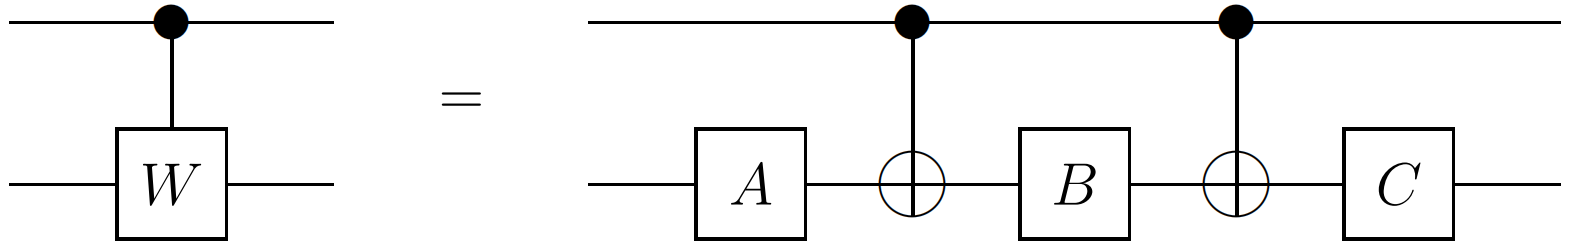
\includegraphics[width=0.5\linewidth]{figure/CCCG_D/CCCG2CCCX.png}
  \caption{控制G门的分解示意图\cite{barenco1995elementary}}
  \label{fig:三组对比}
\end{figure}

% \vspace{0.3cm}

\begin{figure}[H]
  \centering
    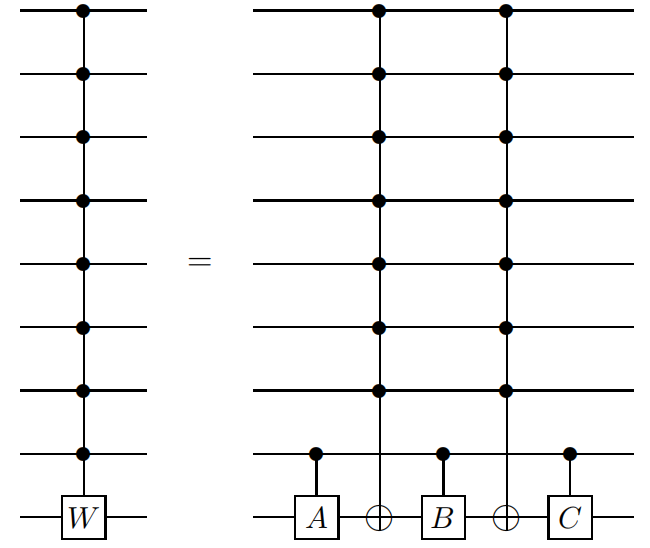
\includegraphics[width=0.5\linewidth]{figure/CCCG_D/CCCG2CCCX_1.png}
  \caption{多控G门的分解示意图\cite{barenco1995elementary}}
  \label{fig:三组对比}
\end{figure}

\subsection{多控Toffoli门的分解}

这里针对多控Toffoli门的分解可以使用借位辅助比特，由于本文中，只要不是$n-1$个控制位的$C^{n-1}NOT$门，均可以使用该方法。

针对 $C^{n}NOT$ 门的分解，只要存在一个辅助比特，就可以进行分解与综合。这里分解综合分为两步，第一步将$C^{n}NOT$缩减到一般的控制位，第二步将后续多控Toffoli门分解到Toffoli门。

第一步分解具体而言：

当$n$为奇数时，可以将 $C^{2n-1}NOT$ 门分解为四个 $C^{n}NOT$ 门：

$$
    C^{2n-1}NOT \quad = \quad 4 \times C^{n}NOT
$$
    
当$n$为偶数时，可以将 $C^{2n}NOT$ 门分解为两个 $C^{n}NOT$ 门和两个 $C^{n+1}NOT$ 门：

$$
    C^{2n}NOT \quad = \quad 2 \times C^{n}NOT + 2 \times C^{n+1}NOT
$$

第二部分解，针对第一步分解后的多控Toffoli门进行处理，如图三红框所示。针对这些门而言，如果其有$m$个控制位，那么我们至少拥有$m-1$个借位辅助比特。然而，其仅需$m-2$个借位辅助比特就可以分解为$4(m-1)$个Toffoli门：
$$
    C^{m}NOT \quad = \quad 4(m-1) \times C^{2}NOT
$$

\vspace{0.3cm}

\begin{figure}[H]
  \centering
    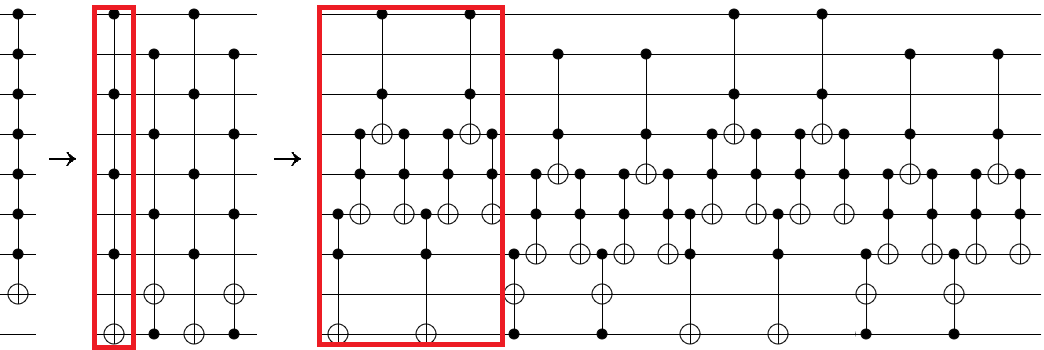
\includegraphics[width=0.9\linewidth]{figure/CCCG_D/all_D_CCCX _1.png}
  \caption{多控Toffoli门的分解示意图\cite{Gidney2015}}
  \label{fig:三组对比}
\end{figure}


%%%%%%%%%%%%%%%%%%%%%%%%%%%%%%%%%%%%%%%%%%
%%%%%%%%%%%%%%%%%%%%%%%%%%%%%%%%%%%%%%%%%%


\section{\heiti 基于AI引导的平行多面体搜索}

第三节所述方法通过逐对合并非零相位实现态制备，其核心优化目标是减少每次合并所需的多控G门控制位数。然而，该贪心策略的局部最优选择并不保证全局最优。近年来，Zheng等\cite{zheng2025cnot}提出了基于平行多面体空间结构的布尔函数合成方法（SSHR），将量子预言机合成问题转化为加权奇偶覆盖问题（Weighted Parity Set Cover Problem, WP-SCP）。本节在此基础上，提出三种基于AI技术的改进策略：基于XOR语义的Beam搜索、基于机器学习的候选排序以及AI剪枝的ILP精确求解方法。

\subsection{\heiti 平行多面体与加权奇偶覆盖}

在布尔函数$F:\{0,1\}^n \to \{0,1\}$的量子线路合成中，\textbf{平行多面体}（parallelotope）是一种几何块结构，定义为$\{0,1\}^n$中由基模式$\mathbf{b}\in\{0,1\}^n$和一组不相交基向量$\{\mathbf{e}_1,\ldots,\mathbf{e}_d\}$确定的子集。其维度为$d$，大小为$2^d$。每个平行多面体对应一组可以同时翻转的变量组合，在量子线路中可通过一次多控操作实现。

将真值表中所有取值为1的最小项集合记为on-set $\mathcal{F}$，取值为0的记为off-set。\textbf{加权奇偶覆盖}要求选择一组平行多面体$\{P_1,\ldots,P_k\}$，使得：
\begin{itemize}[noitemsep,nolistsep]
  \item on-set中的每个最小项被奇数个平行多面体覆盖；
  \item off-set中的每个最小项被偶数个平行多面体覆盖。
\end{itemize}
该问题的目标是最小化所选平行多面体对应的CNOT门总数。当$n$增大时，候选平行多面体数量呈指数增长（$n=4$时为257个，$n=7$时为75{,}905个，$n=8$时为609{,}441个），使得精确求解面临严重挑战。

\subsection{\heiti XOR语义的Beam搜索}
\label{sec:xor-beam}

SSHR-H\cite{zheng2025cnot}采用贪心策略逐个选取平行多面体，使用\textbf{集合减}（set subtract）语义：选定一个平行多面体$P$后，从当前on-set中移除$P$覆盖的所有最小项。然而，这种单调语义限制了搜索空间——仅允许选择完全包含于当前on-set的平行多面体。

我们提出采用\textbf{XOR语义}（又称奇偶更新语义）：选定平行多面体$P$后，对当前覆盖状态执行异或操作，即被覆盖的每个最小项翻转其奇偶性。形式化地，设当前覆盖状态为比特掩码$\mathcal{C}$，则更新规则为：
\begin{equation}
  \mathcal{C} \gets \mathcal{C} \oplus P
\end{equation}
其中$\oplus$表示逐位异或。这意味着原本在on-set中的最小项可能暂时变为off-set，后续通过其他平行多面体的覆盖再次翻转回来。

XOR语义具有两个关键优势：（1）候选集不再受限于当前on-set，所有已枚举的平行多面体均可作为候选，搜索空间大幅扩展；（2）允许"抵消"操作，使得高维平行多面体即便部分覆盖off-set也可被选用，从而可能实现更紧凑的整体覆盖。

在XOR语义下，我们采用\textbf{Beam搜索}策略\cite{lowerre1976harpy}进行求解。设beam宽度为$w$，算法维护$w$个当前最优的部分解。在每一步中，对每个部分解尝试所有候选平行多面体，评估新生成状态的质量，保留最优的$w$个进入下一轮。状态评估函数综合考虑当前on-set的大小和剩余候选的覆盖潜力。

实验结果表明，XOR语义是性能提升的主要因素。如表\ref{tab:xor-vs-monotone}所示，在$n=5$时，XOR Beam相比单调Beam平均减少$10.6\%$的CNOT门；在$n=7$时，对于大规模on-set（$49$--$64$个最小项），改进幅度达到$15.6\%$。

\begin{table}[H]
  \centering
  \caption{XOR语义与单调语义的Beam搜索对比（平均CNOT门数）}
  \label{tab:xor-vs-monotone}
  \setlength{\tabcolsep}{6pt}
  \begin{tabular}{lccc}
    \toprule
    方法 & $n{=}4$ & $n{=}5$ & $n{=}6$ \\
    \midrule
    单调Beam & 20.2 & 41.7 & 62.1 \\
    XOR Beam + 规则排序 & 20.2 & 37.3 & 67.5 \\
    \midrule
    改进率 & 0\% & 10.6\% & $-$8.7\% \\
    \bottomrule
  \end{tabular}
\end{table}

\subsection{\heiti AI引导的候选排序}
\label{sec:ml-ranker}

在Beam搜索中，每一步需要对候选平行多面体进行排序以选择最有潜力的扩展方向。SSHR-H使用基于维度阈值$R=3/4$的手工启发式规则进行排序。我们提出使用机器学习模型替代手工规则，学习候选平行多面体在当前搜索状态下的效用评估。

\subsubsection*{\heiti 特征设计}

对于每个候选平行多面体$P$及当前覆盖状态$\mathcal{C}$，我们提取以下特征：
\begin{enumerate}
  \item 平行多面体维度$d(P)$及其对应的CNOT门成本；
  \item $P$与当前on-set $\mathcal{F}$的交集大小$|P \cap \mathcal{F}|$；
  \item $P$与当前off-set的交集大小$|P \cap (\mathcal{U}\setminus\mathcal{F})|$，其中$\mathcal{U}$为全集；
  \item 覆盖效率：$|P \cap \mathcal{F}|/d(P)$；
  \item 与已选平行多面体集合的冗余度度量。
\end{enumerate}

\subsubsection*{\heiti 模型与训练}

我们采用轻量级的梯度提升决策树（Gradient Boosting Decision Tree, GBDT）\cite{friedman2001greedy}作为排序模型。训练数据通过以下方式生成：在$n=4,5$规模下运行精确ILP求解器获得最优解，将最优解中每一步选择的平行多面体标记为正样本，其余候选标记为负样本。模型输入为上述特征向量，输出为候选的优先级分数。

\subsubsection*{\heiti 实验效果}

表\ref{tab:ml-vs-rule}展示了ML排序与规则排序的直接对比。在$n=5$的100个测试函数中，ML排序在15个函数上优于规则排序，仅在1个函数上劣于规则排序，其余84个函数两者结果相同。在$n=6$的50个测试函数中，ML排序在7个函数上更优，3个函数上更差，40个函数持平。总体而言，ML排序在$n=5$和$n=6$上分别带来约$1\%$--$2\%$的额外CNOT门节省。

\begin{table}[H]
  \centering
  \caption{ML排序与规则排序的直接对比（胜/负/平局）}
  \label{tab:ml-vs-rule}
  \begin{tabular}{lccc}
    \toprule
    变量数$n$ & ML更优 & 规则更优 & 平局 \\
    \midrule
    $n=5$（100个函数） & 15 & 1 & 84 \\
    $n=6$（50个函数） & 7 & 3 & 40 \\
    \bottomrule
  \end{tabular}
\end{table}

\subsection{\heiti AI剪枝的ILP精确求解}
\label{sec:ai-ilp}

加权奇偶覆盖问题可精确建模为整数线性规划（ILP）\cite{gurobi2023}。然而，随着变量数$n$增大，候选平行多面体数量急剧增长（$n=6$时超过10{,}000个），ILP变量数过多导致求解器内存溢出或超时。

我们提出\textbf{AI剪枝策略}：在ILP求解之前，利用训练好的排序模型对所有候选平行多面体进行评分，仅保留得分最高的$K$个候选（$K \ll $ 总候选数）以及满足特定"安全单例"条件的候选，构建缩小后的ILP实例。安全单例是指那些覆盖了仅被一个候选平行多面体覆盖的最小项（即必选候选），确保这些关键覆盖不被遗漏。

设原始候选集为$\mathcal{P}$，AI剪枝后的候选集为$\mathcal{P}' \subset \mathcal{P}$，则：
\begin{equation}
  \mathcal{P}' = \mathrm{Top\text{-}}K(\mathrm{Score}(\mathcal{P})) \cup \mathrm{Singletons}(\mathcal{P}, \mathcal{F})
\end{equation}
其中$\mathrm{Score}(\cdot)$为ML排序模型的评分函数，$\mathrm{Singletons}(\cdot)$为安全单例筛选函数。

如表\ref{tab:ai-ilp}所示，在$n=4$时，AI剪枝ILP在保持与精确ILP完全相同的解质量（平均16.6个CNOT门）的前提下，将求解速度提升了128倍（从4.6秒降至34毫秒）。在$n=5$时，AI剪枝ILP的平均CNOT门数为34.4，仅比精确ILP的26.8高，但避免了$n \ge 6$时的内存溢出问题。

\begin{table}[H]
  \centering
  \caption{AI剪枝ILP与精确ILP的对比}
  \label{tab:ai-ilp}
  \setlength{\tabcolsep}{6pt}
  \begin{tabular}{lccccc}
    \toprule
    \multirow{2}{*}{方法} & \multicolumn{2}{c}{$n{=}4$} & \multicolumn{2}{c}{$n{=}5$} & \multirow{2}{*}{$n{=}6$} \\
    \cmidrule(lr){2-3} \cmidrule(lr){4-5}
    & CNOT & 时间 & CNOT & 时间 & \\
    \midrule
    精确ILP & 16.6 & 4.6s & 26.8 & 0.3s & OOM \\
    AI剪枝ILP & 16.6 & 34ms & 34.4 & 3s & --- \\
    \midrule
    加速比 & \multicolumn{2}{c}{128$\times$} & \multicolumn{2}{c}{---} & --- \\
    \bottomrule
  \end{tabular}
\end{table}

此外，我们设计了\textbf{混合XOR+ILP策略}：先用XOR Beam搜索生成初始解，再对剩余未覆盖部分调用AI剪枝ILP进行精确求解。该策略在$n=5$时取得了34.8个CNOT门的平均结果，介于纯Beam搜索和精确ILP之间，但能够发现Beam搜索和ILP单独均无法找到的优质解。


%%%%%%%%%%%%%%%%%%%%%%%%%%%%%%%%%%%%%%%%%%
%%%%%%%%%%%%%%%%%%%%%%%%%%%%%%%%%%%%%%%%%%


\section{\heiti 数值实验和应用案例}

在数值实验这一部分，我们首先在全连接结构上，针对随机态进行多次实验测算我们的算法线路长度，接着在Heavy-hex,Square两个特定结构上进行MAPPING，同样对随机态进行多次实验测算我们的线路长度。此外，我们给出了一个稀疏量子态制备的案例。

\subsection{随机态}

针对本文算法在$qubits$数量$N$在$10-50$，非零系数的数量$S$在$N^1-N^{1.5}$的范围内进行数值实验 结果在下表1。

\begin{table}[H]
  \centering
  \caption{量子态稀疏相位数量S作为Qubits数量N的幂函数时，不同N值下电路规模数据表，其中线路复杂度系数为CNOT门数与SN的比值。值得注意的是，当N的值较小时，其幂值差异较小，我们这里四舍五入处理}
  
  \label{tab:data}
  \setlength{\tabcolsep}{6pt} % 调整列间距
  \begin{tabular}{
    l % S=N^k 列
    S[table-format=2.2] % N=10 CNOT
    S[table-format=1.4] % N=10 系数
    S[table-format=3.2] % N=20 CNOT
    S[table-format=1.4] % N=20 系数
    S[table-format=3.2] % N=30 CNOT
    S[table-format=1.4] % N=30 系数
    S[table-format=4.2] % N=40 CNOT
    S[table-format=1.4] % N=40 系数
    S[table-format=4.2] % N=50 CNOT
    S[table-format=1.4] % N=50 系数
  }
    \toprule
    \multirow{2}{*}{$S=N^k$} & \multicolumn{2}{c}{$qubit=10$} & \multicolumn{2}{c}{$qubit=20$} & \multicolumn{2}{c}{$qubit=30$} & \multicolumn{2}{c}{$qubit=40$} & \multicolumn{2}{c}{$qubit=50$} \\
    \cmidrule(lr){2-3} \cmidrule(lr){4-5} \cmidrule(lr){6-7} \cmidrule(lr){8-9} \cmidrule(lr){10-11}
    & {CNOT} & {系数} & {CNOT} & {系数} & {CNOT} & {系数} & {CNOT} & {系数} & {CNOT} & {系数} \\
    \midrule
    % S=N^1
    $S=N^1$ & 41.13 & 0.4113 & 182.60 & 0.4565 & 422.98 & 0.4700 & 753.36 & 0.4709 & 1173.75 & 0.4695 \\
    % S=N^1.1
    $S=N^{1.1}$ & 55.50 & 0.4408 & 265.48 & 0.4919 & 619.55 & 0.4899 & 1140.79 & 0.4930 & 1826.11 & 0.4940 \\
    % S=N^1.2
    $S=N^{1.2}$ & 78.32 & 0.4942 & 382.43 &0.5251 & 939.05 & 0.5285 & 1792.15 &0.5356 & 2973.58 &0.5439 \\
    % S=N^1.3
    $S=N^{1.3}$ & 111.17 & 0.5572 & 557.58 & 0.5675 & 1450.87 &0.5810 & 2859.18 &0.5908 & 4833.90 & 0.5980 \\
    % S=N^1.4
    $S=N^{1.4}$ & 154.99 & 0.6170 &834.83 &0.6297 & 2279.77 & 0.6498 & 4626.86 & 0.6612 & 8066.03 & 0.6747 \\
    % S=N^1.5
    $S=N^{1.5}$ &216.51 & 0.6846 &1260.93 & 0.7049 &3608.86 & 0.7321 & 7623.90 & 0.7534 & 13616.88 & 0.7703 \\
    \bottomrule
  \end{tabular}
\end{table}


对图表进行分析可知，随着$S$数量增加，系数存在明显的上升。随这个$N$的增加，系数呈现先上升，最后趋于稳定的趋势。
Gleinig与Hoefler\cite{gleinig2021efficient}在2021年DAC上提出的相位缩减方法作为当前不使用辅助比特的最优方法，具有重要参考价值。为展示本文算法优势，我们对本文提出的算法与其进行了数值测试与性能比对。
\par
我们均匀随机抽取$k$个长度为$n$的二进制字符串。由于振幅对本文算法与Gleinig\cite{gleinig2021efficient}提出的算法均不影响电路规模，因此无需对振幅进行采样。需要说明的是，由于CNOT门数量通常能有效表征电路规模，故实验中以CNOT门数量而非电路规模作为计量指标，具体结果如图四至图六所示。

\begin{figure}[H]
  \centering

  % 第一行：S=N
  \begin{subfigure}[b]{.494\linewidth}
    \centering
    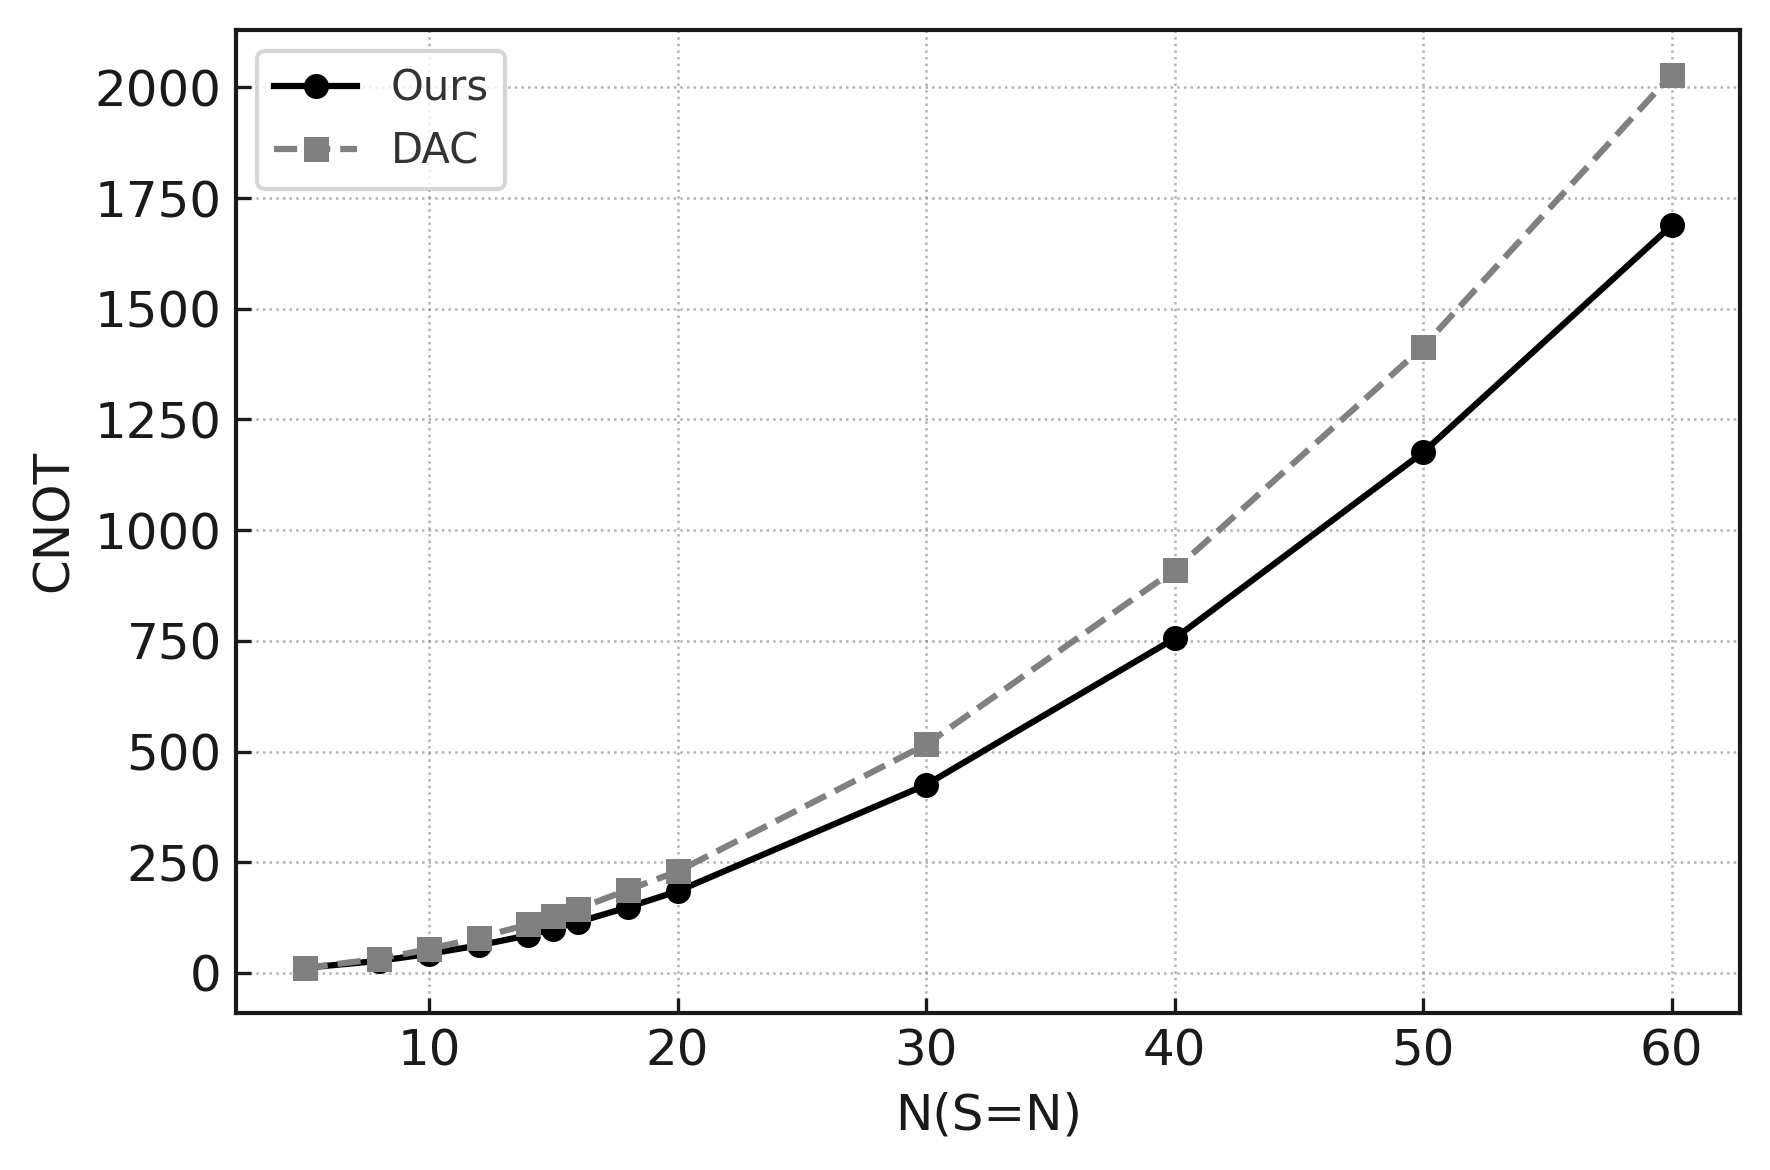
\includegraphics[width=\linewidth]{figure/cnot_vs_n_total.png}
    \caption{CNOT门数}
    \label{fig:S=N的门数}
  \end{subfigure}
  \hfill
  \begin{subfigure}[b]{.494\linewidth}
    \centering
    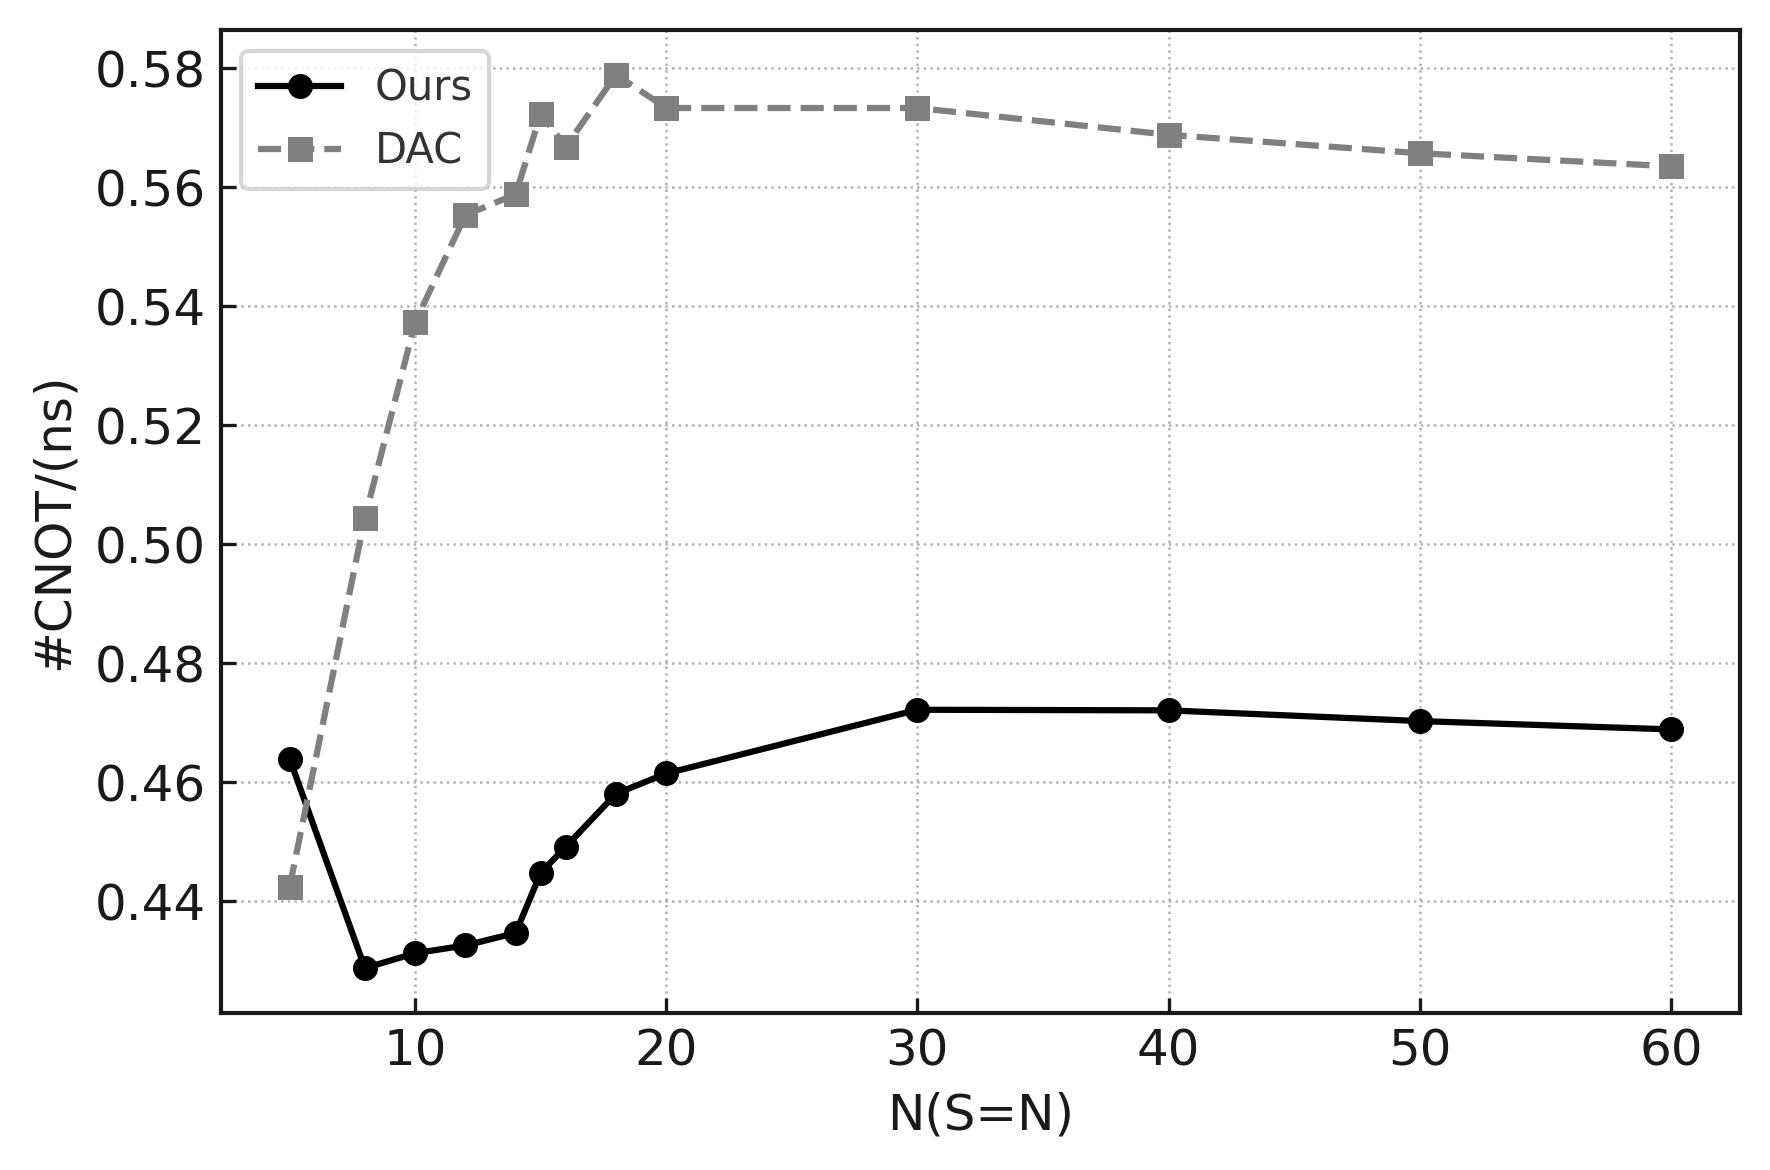
\includegraphics[width=\linewidth]{figure/cnot_vs_n_grid.png}
    \caption{CNOT门系数}
    \label{fig:S=N的系数}
  \end{subfigure}

  \caption{当态稀疏相位数量S等于Qubits数量N时，（a）CNOT门数与S，N的变化关系对比图，（b）线路复杂度系数与S，N的变化关系对比图，其中线路复杂度系数为CNOT门数与SN的比值}
  \label{fig:三组对比}
\end{figure}

  % \vspace{0.5em} % 行间距微调


\begin{figure}[H]
  \centering
  % 第二行：固定N
  \begin{subfigure}[b]{.45\linewidth}
    \centering
    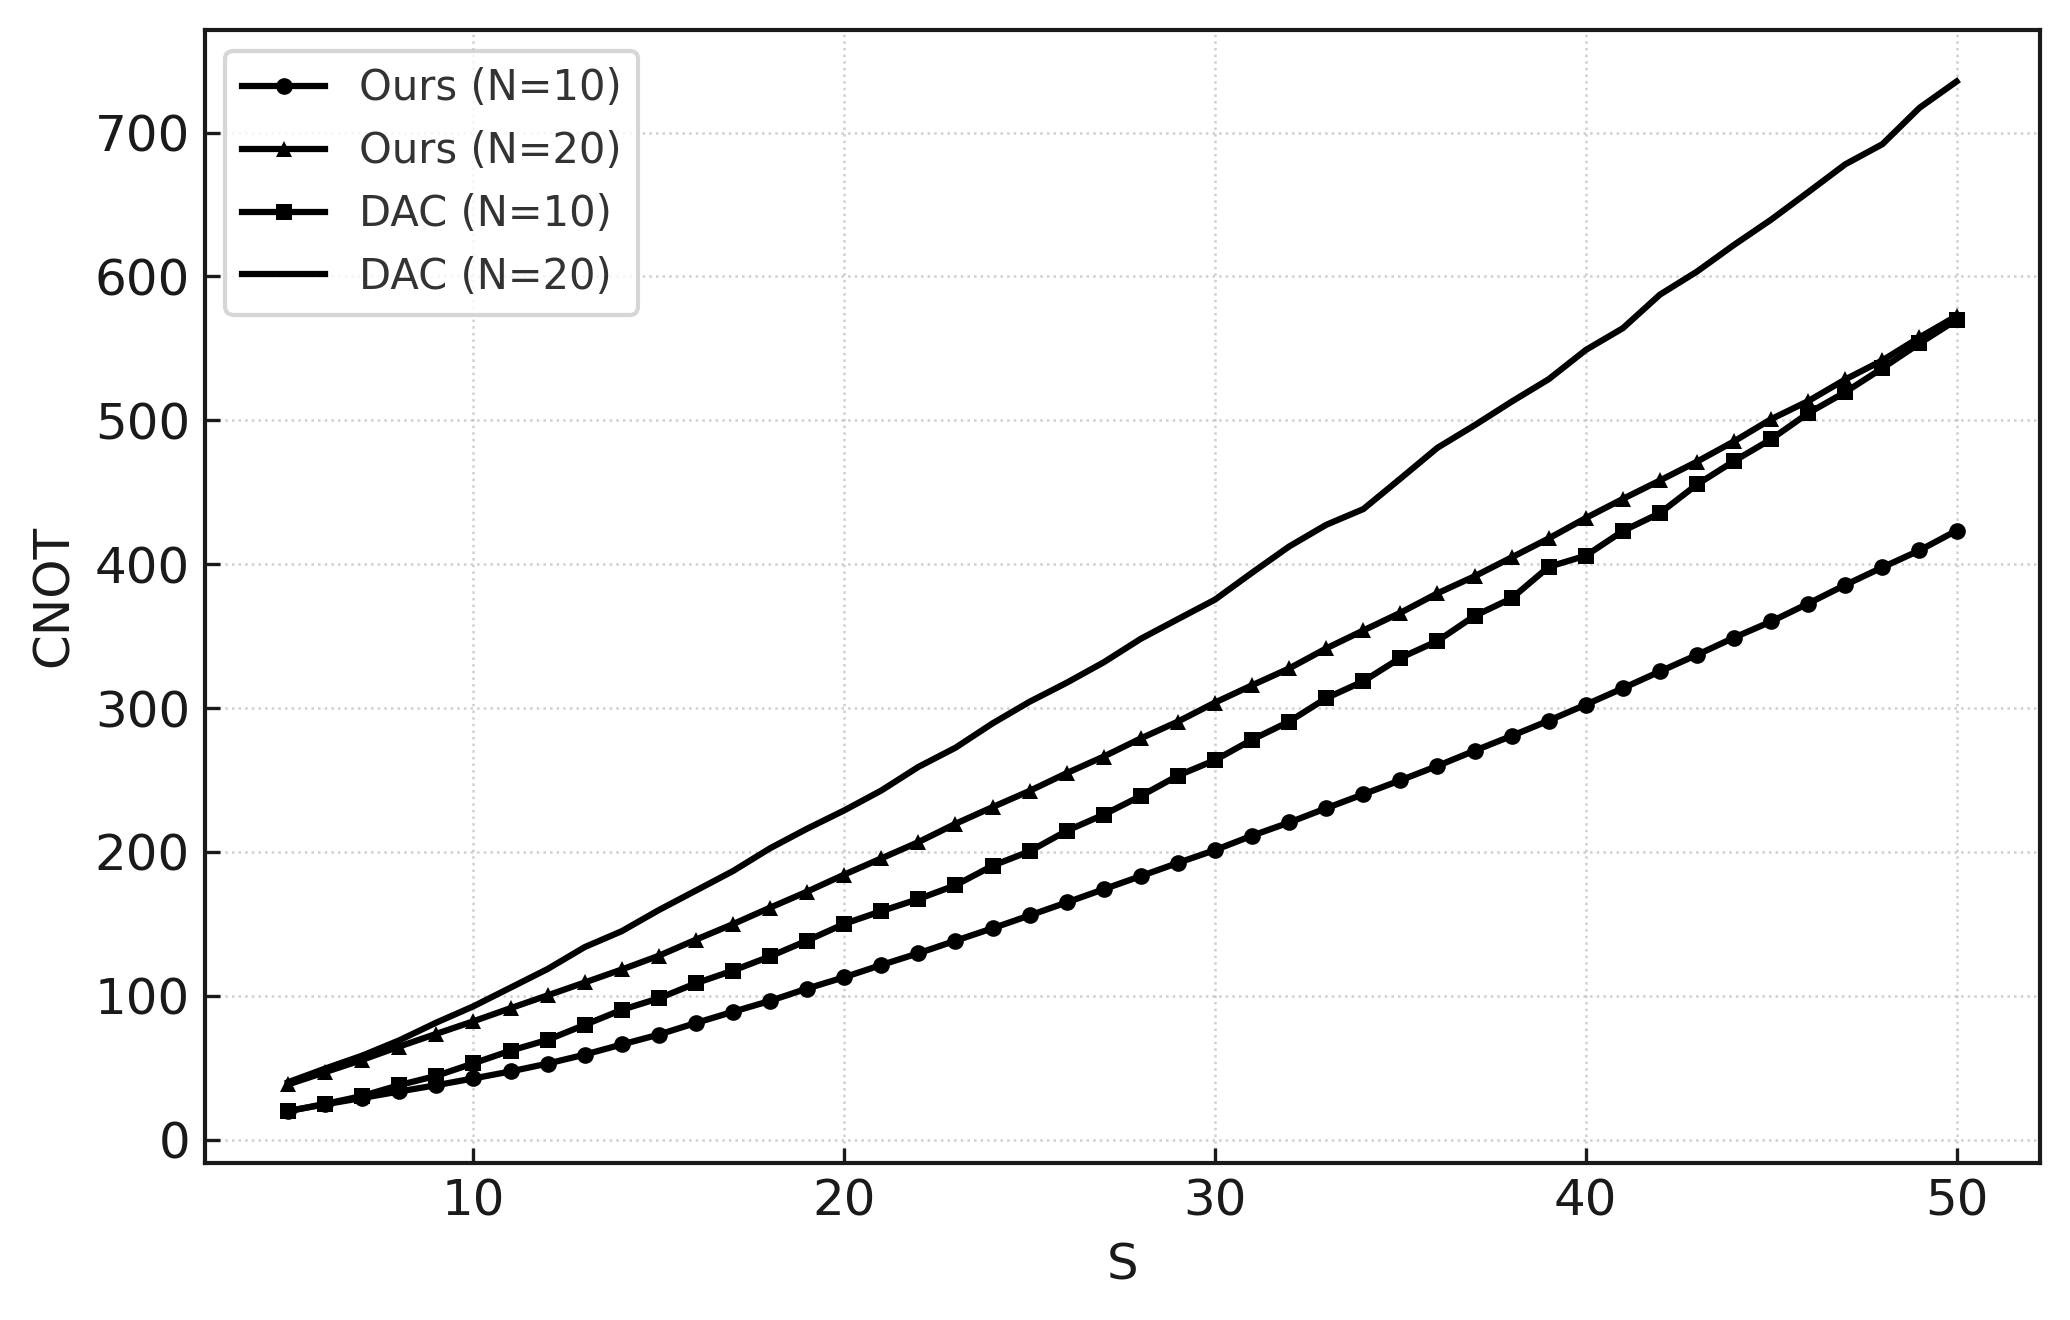
\includegraphics[width=\linewidth]{figure/cnot_total_vs_S_N10N20_allblack.png}
    \caption{CNOT门数}
    \label{fig:固定N门数}
  \end{subfigure}
  \hfill
  \begin{subfigure}[b]{.45\linewidth}
    \centering
    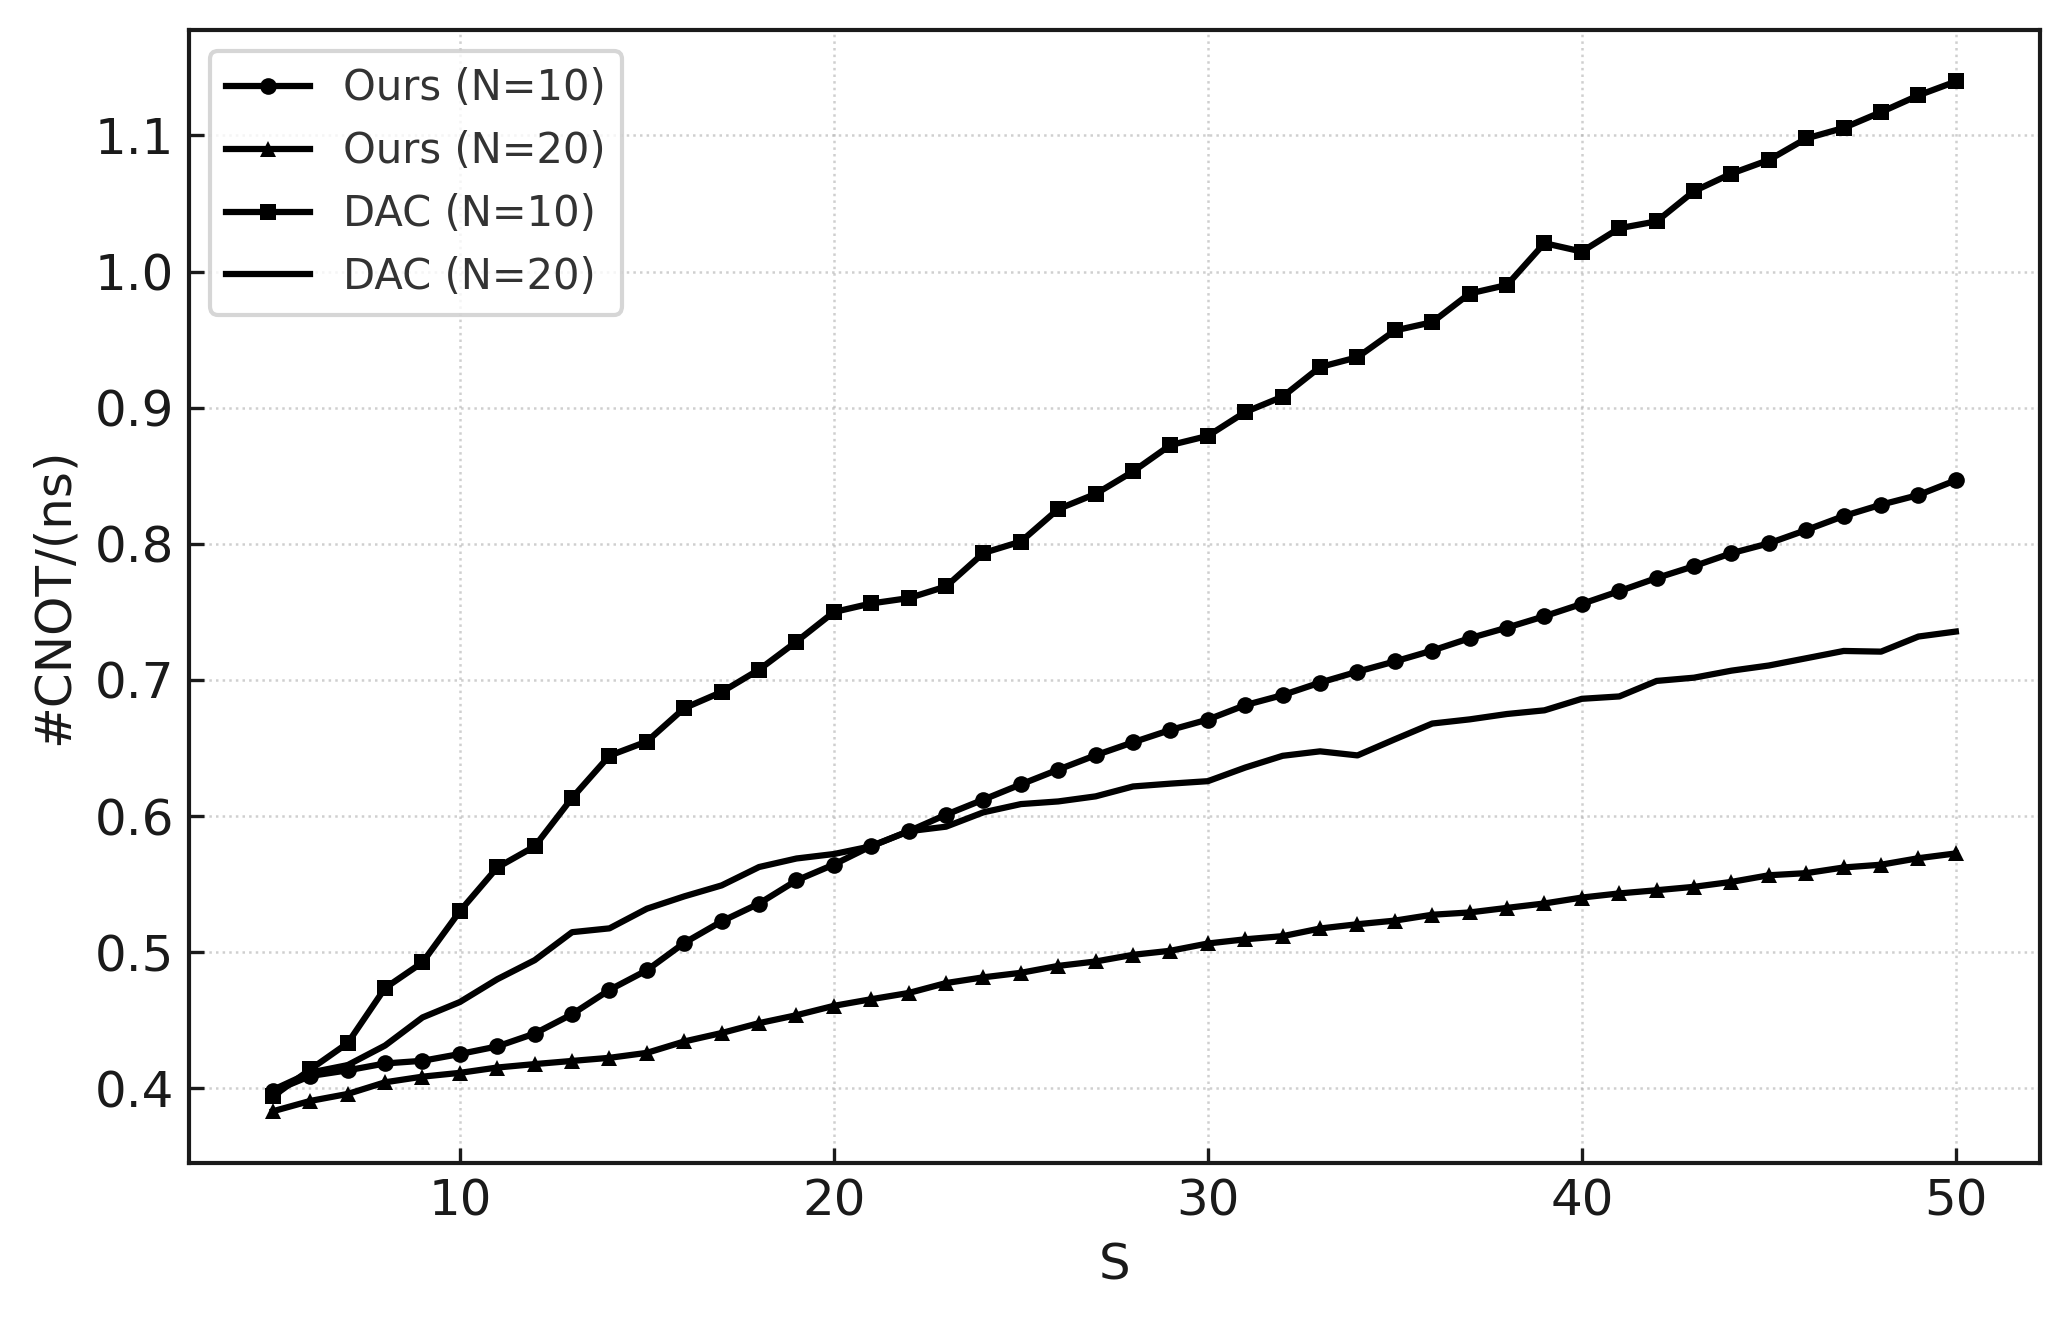
\includegraphics[width=\linewidth]{figure/cnot_per_ns_vs_S_N10N20_allblack.png}
    \caption{CNOT门系数}
    \label{fig:固定N系数}
  \end{subfigure}

  \caption{当Qubits数量N固定时，（a）CNOT门数与S的变化关系对比图，（b）线路复杂度系数与S的变化关系对比图，其中线路复杂度系数为CNOT门数与SN的比值}
  \label{fig:三组对比}
\end{figure}

  % \vspace{0.5em} % 行间距微调


\begin{figure}[H]
  \centering
  % 第三行：固定S
  \begin{subfigure}[b]{.45\linewidth}
    \centering
    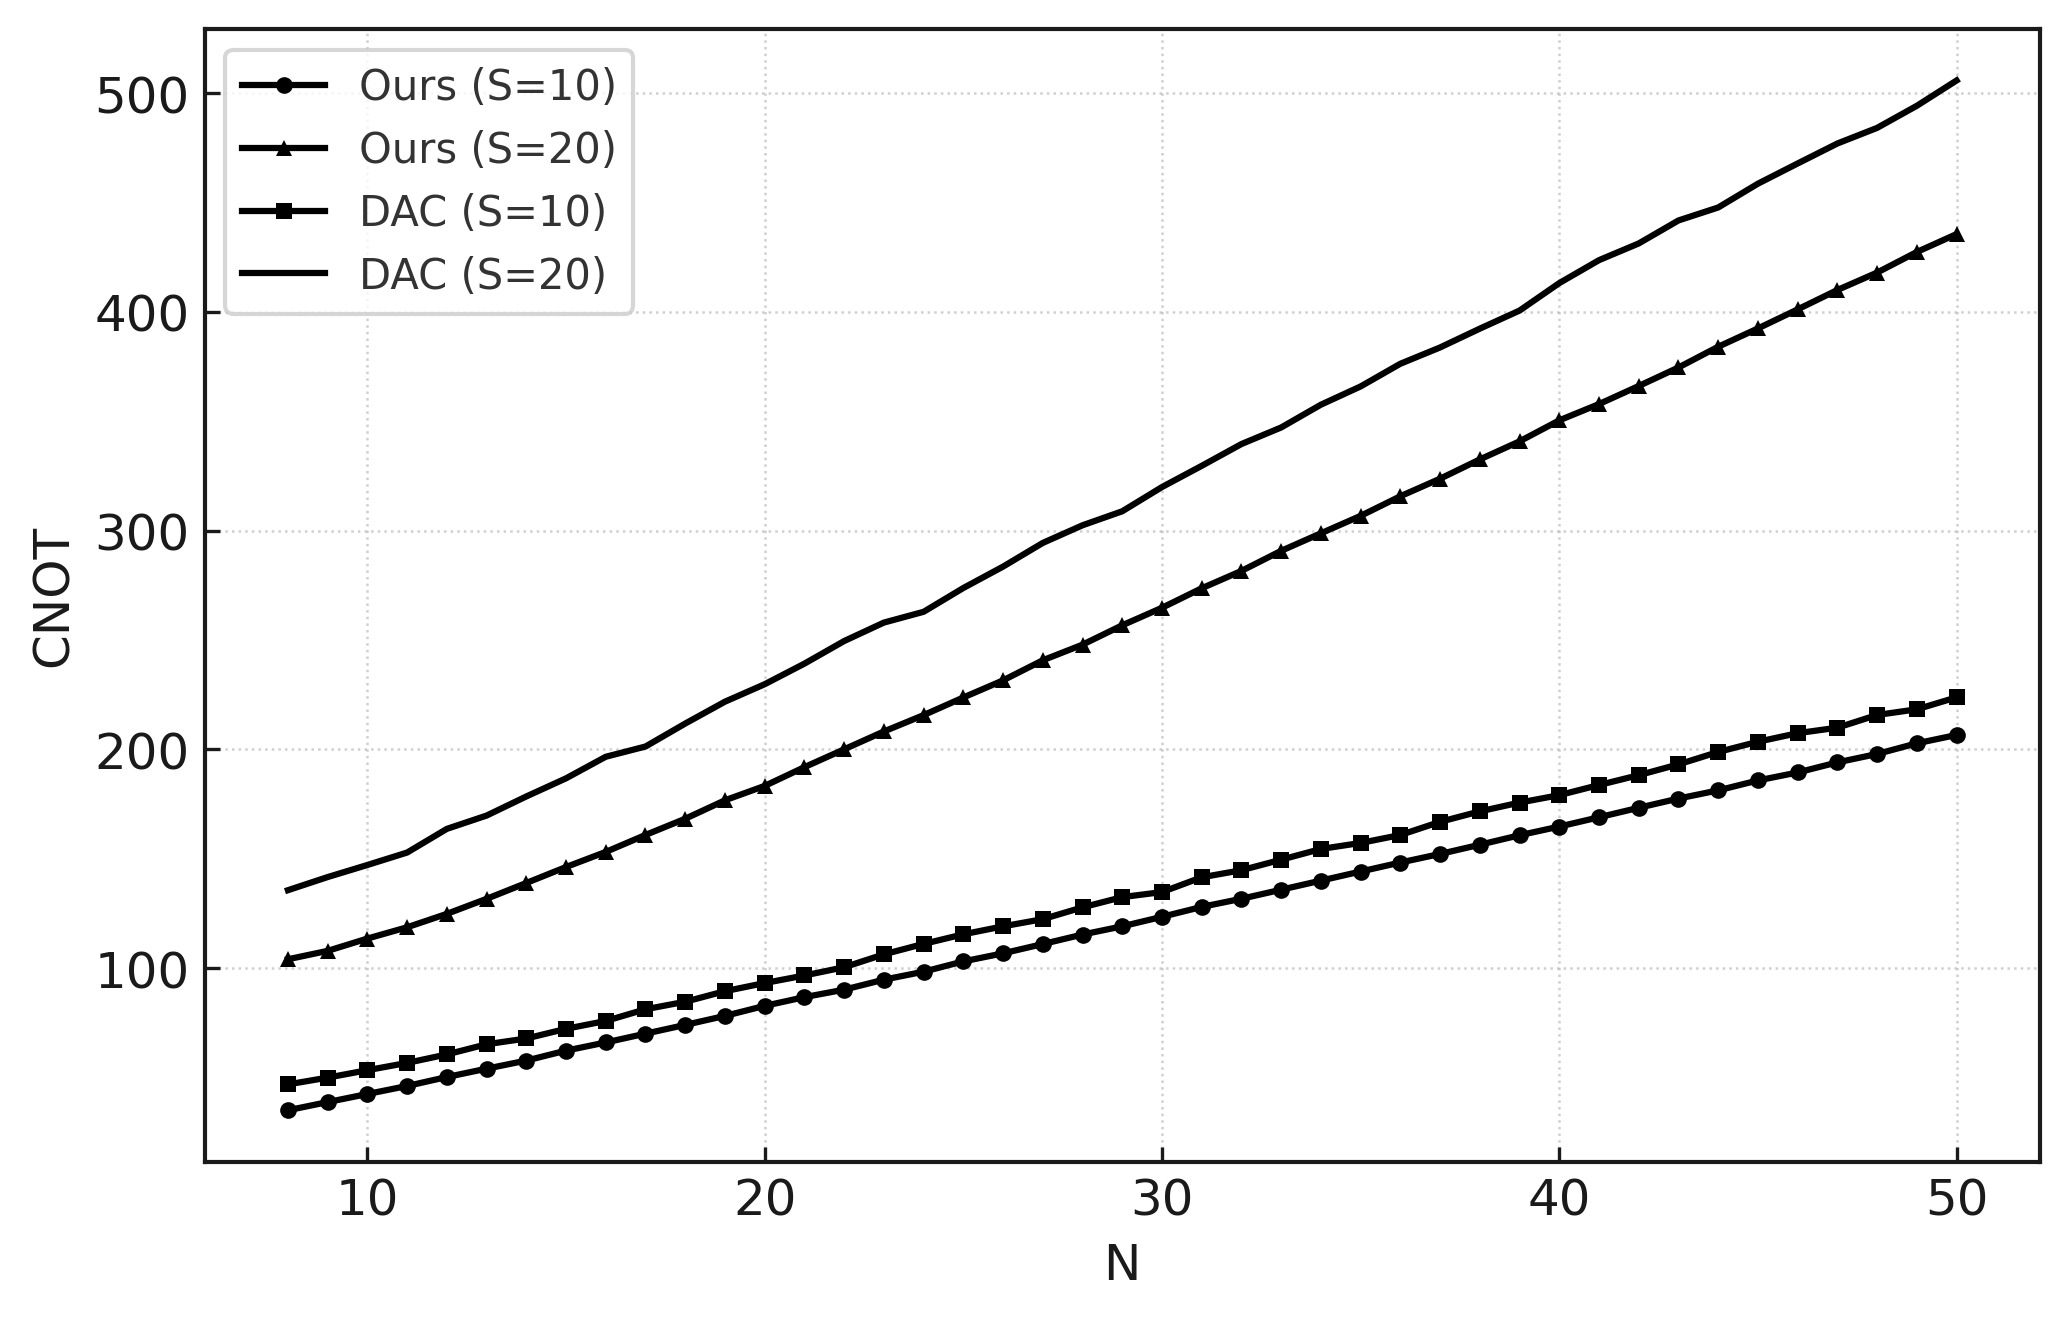
\includegraphics[width=\linewidth]{figure/cnot_total_vs_N_S10S20_allblack.png}
    \caption{CNOT门数}
    \label{fig:比特增长门数}
  \end{subfigure}
  \hfill
  \begin{subfigure}[b]{.45\linewidth}
    \centering
    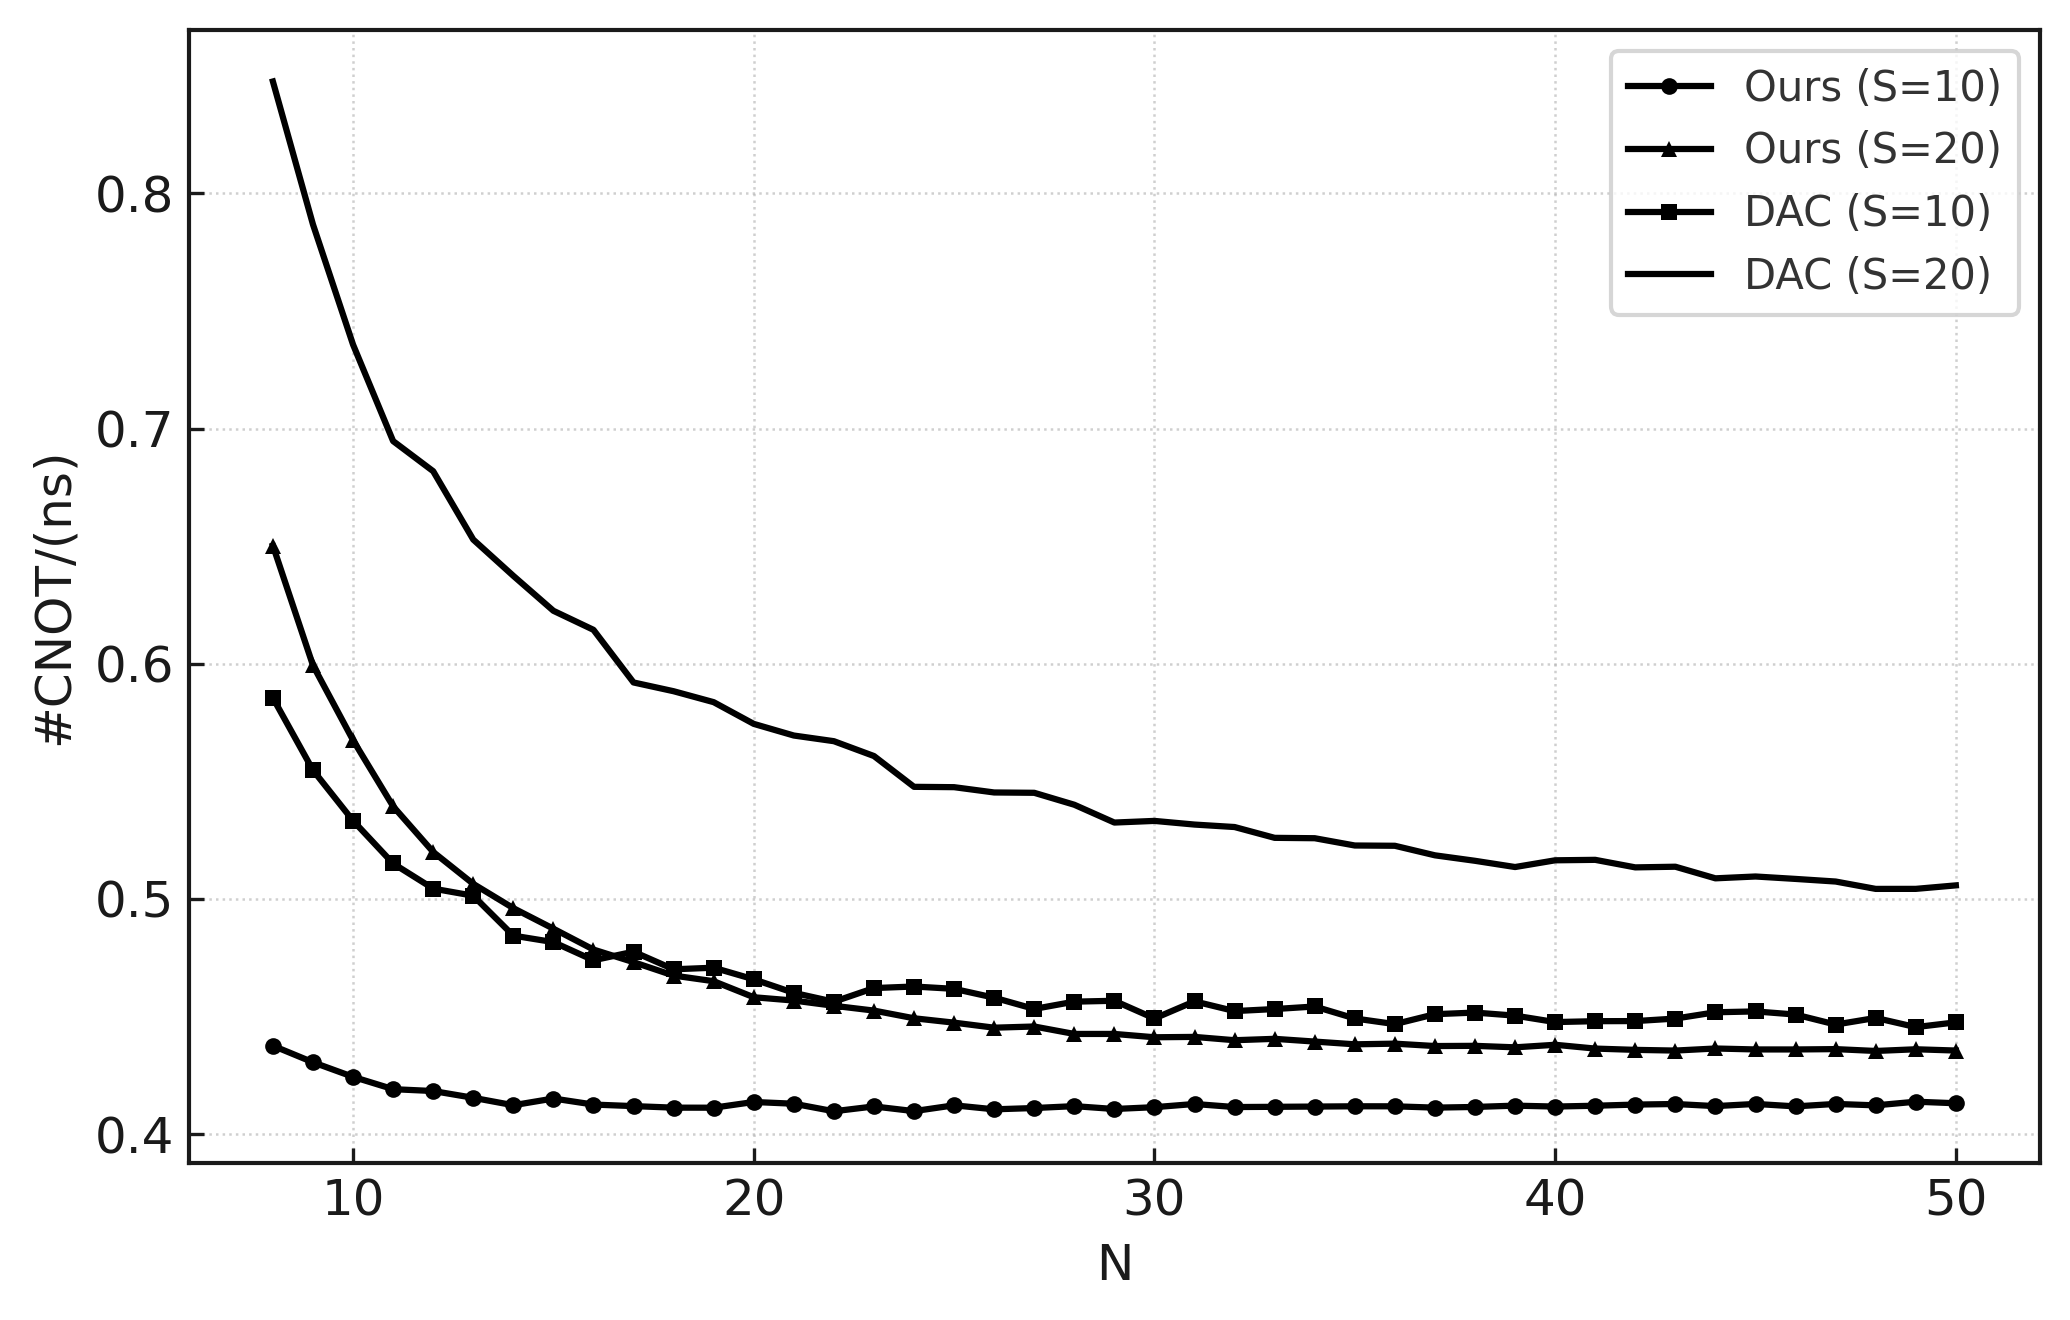
\includegraphics[width=\linewidth]{figure/cnot_per_ns_vs_N_S10S20_allblack.png}
    \caption{CNOT门系数}
    \label{fig:比特增长系数}
  \end{subfigure}

  \caption{当态稀疏相位数量S不变时，（a）CNOT门数与N的变化关系对比图，（b）线路复杂度系数与N的变化关系对比图，其中线路复杂度系数为CNOT门数与SN的比值}
  \label{fig:三组对比}
\end{figure}

\par
特别的，在比特数量和量子非零相位数量都为$10$时，本文算法相较于Gleinig\cite{gleinig2021efficient}提出的算法可以节省$19.73\%$的$CNOT$门；当比特数量和量子非零相位数量都为$15$时，我们算法可以节省$22.28\%$的$CNOT$门；当比特数量和量子非零相位数量都为$30$时，我们算法可以节省$17.63\%$的$CNOT$门；当比特数量和量子非零相位数量都为$50$时，我们算法可以节省$16.79\%$的$CNOT$门。并且随着非零相位数量的增加，我们的算法会表现出更大的优势。当在比特数量为$15$非零相位数量为$20$时,我们算法可以节省$21.19\%$的$CNOT$门；当在比特数量为$15$非零相位数量为$50$时,我们算法可以节省$20.40\%$的$CNOT$门；当在比特数量为$15$非零相位数量为$50$时,我们算法可以节省$23.28\%$的$CNOT$门。\par

\subsection{\heiti 基于AI引导的平行多面体搜索实验}

为验证第四节所述方法的有效性，我们在$n=4$至$n=7$的布尔函数上进行了系统性实验。对于每个$n$值，随机选取一定数量的布尔函数作为测试集，对比不同方法的平均CNOT门数和运行时间。所有实验在同一台配备Intel i9处理器和32GB内存的机器上完成。

\subsubsection*{\heiti 方法综合对比}

表\ref{tab:ai-sshr-comparison}汇总了各方法在不同规模下的平均CNOT门数。其中SSHR-H为原始贪心算法\cite{zheng2025cnot}，单调Beam和XOR Beam为本文第四节提出的Beam搜索方法，AI剪枝ILP和精确ILP为基于整数规划的求解方法。

\begin{table}[H]
  \centering
  \caption{各方法平均CNOT门数对比}
  \label{tab:ai-sshr-comparison}
  \setlength{\tabcolsep}{5pt}
  \begin{tabular}{lcccc}
    \toprule
    方法 & $n{=}4$ & $n{=}5$ & $n{=}6$ & $n{=}7$ \\
    \midrule
    SSHR-H（贪心） & 19.3 & 42.4 & 71.1 & 131 \\
    单调Beam & 20.2 & 41.7 & 62.1 & --- \\
    XOR Beam + 规则排序 & 20.2 & 37.3 & 67.5 & 125 \\
    XOR Beam + ML排序 & 20.2 & 36.8 & 67.1 & --- \\
    AI剪枝ILP & 16.6 & 34.4 & --- & --- \\
    精确ILP & 16.6 & 26.8 & OOM & OOM \\
    混合XOR+ILP & --- & 34.8 & 71.2 & --- \\
    \bottomrule
  \end{tabular}
\end{table}

从表中可以得出以下观察：
\begin{enumerate}
  \item \textbf{XOR语义是性能提升的主要因素}。在$n=5$时，XOR Beam（37.3）相比单调Beam（41.7）减少了$10.6\%$的CNOT门，相比SSHR-H（42.4）减少了$12.0\%$。这一改进源于XOR语义允许候选集扩展至全部已枚举的平行多面体，而非仅限于当前on-set的子集。
  \item \textbf{ML排序带来额外改进}。在XOR语义基础上，ML排序在$n=5$时将平均CNOT门数从37.3进一步降低至36.8（减少$1.3\%$），在$n=6$时从67.5降至67.1（减少$0.6\%$）。尽管改进幅度较小，但ML排序在大规模函数上的优势更为稳定。
  \item \textbf{AI剪枝ILP在可承受范围内接近精确最优}。在$n=4$时，AI剪枝ILP与精确ILP获得完全相同的解质量（16.6个CNOT门），但速度提升128倍。在$n=5$时，AI剪枝ILP（34.4）与精确ILP（26.8）存在差距，这是因为剪枝过程移除了部分最优候选。
  \item \textbf{$n=7$规模可行}。得益于平行多面体枚举的高效实现，$n=7$时75{,}905个候选的枚举仅需2.6秒。XOR Beam在$n=7$时平均125个CNOT门，相比SSHR-H的131个减少$4.6\%$。
\end{enumerate}

\subsubsection*{\heiti 不同on-set规模下的性能分析}

表\ref{tab:n7-onset}进一步分析了$n=7$时不同on-set规模下SSHR-H与XOR Beam的性能差异。实验选取50个随机布尔函数，按on-set大小分为小（4--16）、中（17--48）、大（49--64）三组。

\begin{table}[H]
  \centering
  \caption{$n=7$时不同on-set规模下的CNOT门数对比（50个函数）}
  \label{tab:n7-onset}
  \begin{tabular}{lccc}
    \toprule
    on-set规模 & SSHR-H & XOR Beam & 改进率 \\
    \midrule
    小（4--16） & 81.8 & 83.6 & $-$2.2\% \\
    中（17--48） & 151.1 & 141.1 & $+$6.6\% \\
    大（49--64） & 209.8 & 177.0 & $+$15.6\% \\
    \bottomrule
  \end{tabular}
\end{table}

可以看出，XOR语义在大规模on-set上的优势最为显著。当on-set较小时，贪心策略已接近最优，XOR语义的搜索空间扩展反而引入了少量额外开销。随着on-set规模增大，XOR语义允许的高维平行多面体"部分覆盖再抵消"策略发挥了越来越重要的作用，在大规模on-set上实现了$15.6\%$的CNOT门节省。

\subsubsection*{\heiti 各方法运行时间}

表\ref{tab:ai-sshr-speed}列出了各方法的运行时间范围。SSHR-H贪心方法速度最快，在毫秒级完成。XOR Beam在$n=7$时需要约54毫秒，仍远快于ILP方法。精确ILP在$n=4$时需要数秒，在$n \ge 6$时因内存溢出而无法运行。AI剪枝ILP在$n=4$时仅需34毫秒，成功将精确求解的时间降低至可接受范围。

\begin{table}[H]
  \centering
  \caption{各方法运行时间范围}
  \label{tab:ai-sshr-speed}
  \setlength{\tabcolsep}{5pt}
  \begin{tabular}{lcccc}
    \toprule
    方法 & $n{=}4$ & $n{=}5$ & $n{=}6$ & $n{=}7$ \\
    \midrule
    SSHR-H & 0.1ms & 0.3ms & 3ms & 11ms \\
    单调Beam & 3ms & 8ms & 70ms & --- \\
    XOR Beam + 规则 & 2ms & 7ms & 25ms & 54ms \\
    XOR Beam + ML & 11ms & 24ms & 56ms & 98ms \\
    AI剪枝ILP & 34ms & 3s & --- & --- \\
    精确ILP & 4.6s & 0.3s & OOM & OOM \\
    \bottomrule
  \end{tabular}
\end{table}

综合以上实验结果，本节提出的AI引导策略在保持合理运行时间的前提下，有效降低了布尔函数合成的CNOT门开销。其中XOR语义的贡献最为显著（$10\%$--$15\%$的CNOT门节省），ML排序提供$1\%$--$2\%$的额外改进，AI剪枝ILP则在精确性与效率之间取得了良好平衡。
\newpage

\subsection{特定结构的MAPPING}
考虑算法在 NISQ 设备上的适配性，我们将全连接结构的量子线路通过增加线路局部性的方式进行重写与映射：在保持逻辑功能等价的前提下，优先将远距离的两比特相互作用转化为近邻交互，最小化线路长度，进而降低误差、提升在噪声环境下的可执行性。基于这一流程，我们将原始线路分别映射到两类代表性的硬件耦合图，Heavy-Hex与 Square\_25,其结构示意如图\ref{fig:示意图}所示。\par
\begin{figure}[H]
  \centering
  \begin{subfigure}[b]{.55\linewidth}
    \centering
    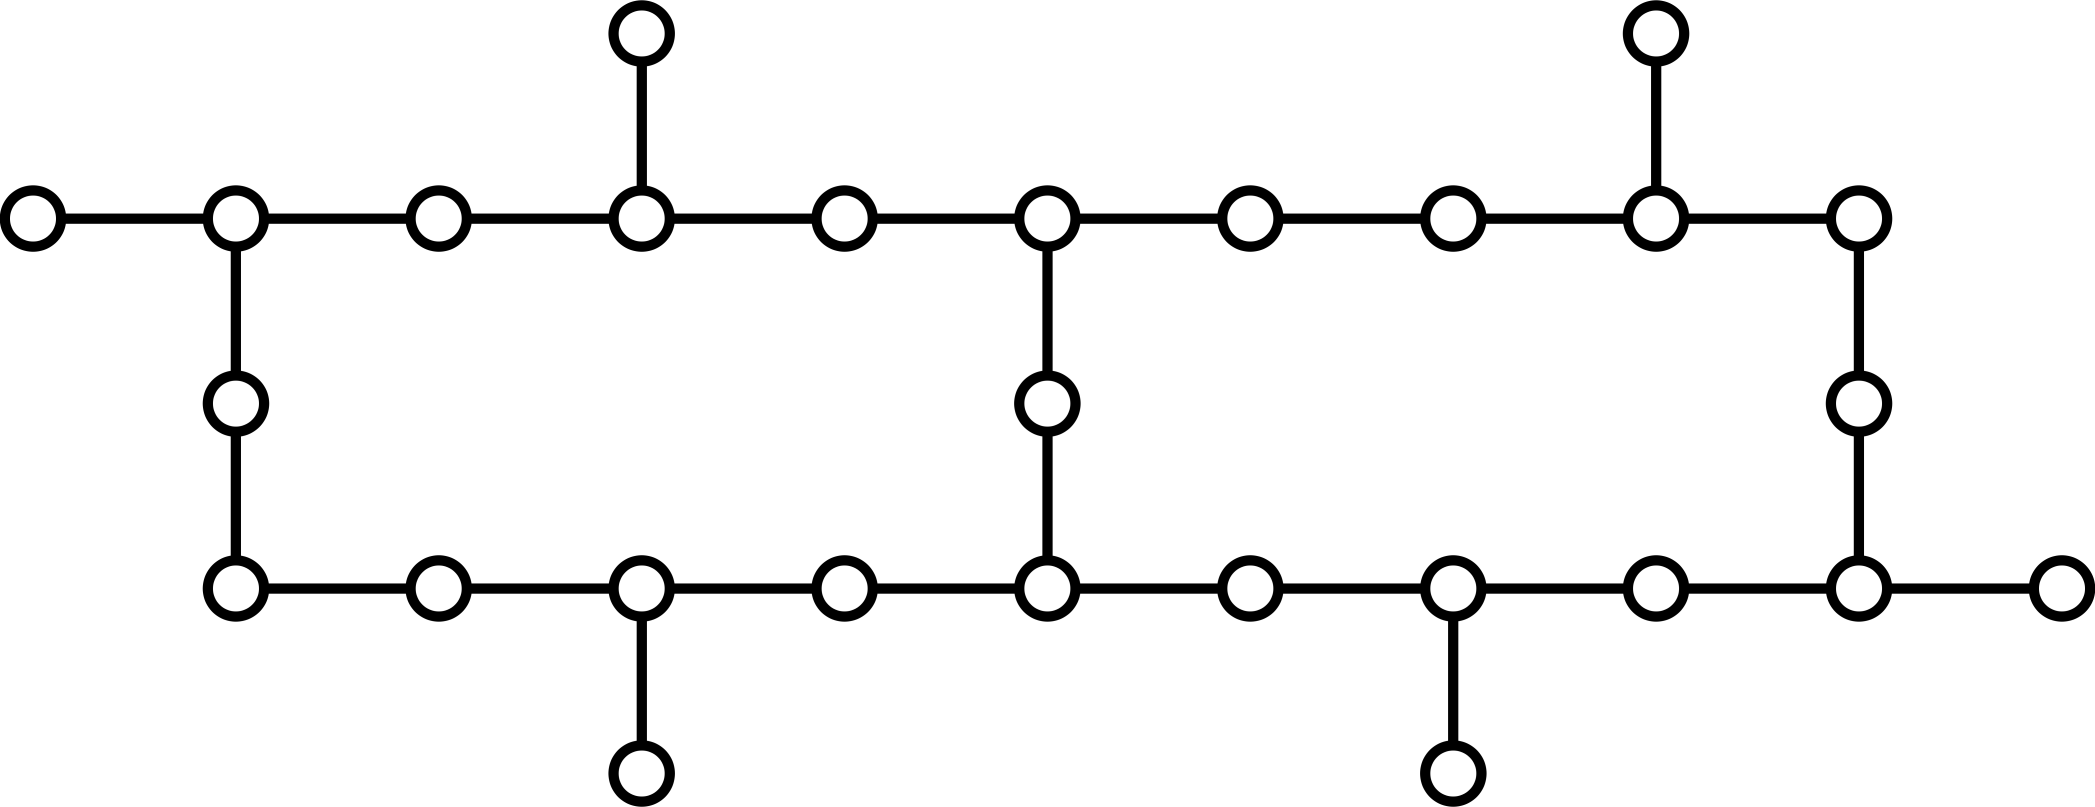
\includegraphics[width=\linewidth]{figure/heavyhex.png}
    \caption{Heavy-Hex结构示意图}
    \label{fig:Heavy-Hex结构}
  \end{subfigure}
  \hfill
  \begin{subfigure}[b]{.4\linewidth}
    \centering
    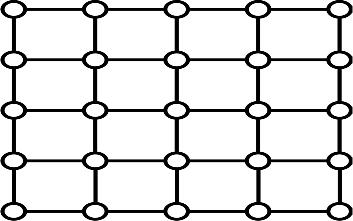
\includegraphics[width=\linewidth]{figure/square.png}
    \caption{Square\_25结构示意图}
    \label{fig:Square结构}
  \end{subfigure}

  \caption{两种特定结构示意图}
  \label{fig:示意图}
\end{figure}

表\ref{table:Heavy10}和表\ref{table:Heavy20}为我们算法在Heavy-Hex上映射的线路长度结果。在该拓扑下，我们的方法相较于目前最优方法\cite{zou2024lightsabre,gleinig2021efficient}在量子比特规模为10和20时均取得显著优势：当 $qubit{=}10$ 时平均节省 19.70\%的线路长度，当 $qubit{=}20$ 时平均节省15.65\%的线路长度；整体节省率随 $S$ 增大呈上升趋势，最高可以节省32.18\%的线路长度，显示出良好的可扩展性与稳健性。

\begin{table}[H]
  \centering
  \caption{Heavy-Hex 实验结果（qubit=10）}
  \label{table:Heavy10}
  \setlength{\tabcolsep}{4pt}
  \resizebox{\textwidth}{!}{%
  \begin{tabular}{l*{20}{r}}
    \toprule
    S & 5 & 10 & 15 & 20 & 25 & 30 & 35 & 40 & 45 & 50 & 55 & 60 & 65 & 70 & 75 & 80 & 85 & 90 & 95 & 100 \\
    \midrule
    DAC   & 1.024 & 1.3327 & 1.5760 & 1.6210 & 1.6883 & 1.7927 & 1.9324 & 2.0742 & 2.2524 & 2.4312 & 2.4646 & 2.6772 & 2.7513 & 2.9855 & 3.1535 & 3.3013 & 3.5546 & 3.6488 & 3.7862 & 3.9236 \\
    Ours  & 1.049 & 1.3840 & 1.3393 & 1.5288 & 1.5450 & 1.5690 & 1.6441 & 1.6615 & 1.7908 & 1.8495 & 1.9586 & 2.0004 & 2.0737 & 2.1974 & 2.2417 & 2.3347 & 2.4635 & 2.5174 & 2.6252 & 2.6610 \\
    Reduce& -0.0244 & -0.0385 & 0.1502 & 0.0569 & 0.0849 & 0.1248 & 0.1492 & 0.1990 & 0.2050 & 0.2393 & 0.2053 & 0.2528 & 0.2463 & 0.2640 & 0.2891 & 0.2928 & 0.3070 & 0.3101 & 0.3067 & 0.3218 \\
    \bottomrule
  \end{tabular}%
  }
\end{table}
\begin{table}[H]
  \centering
  \caption{Heavy-Hex 实验结果（qubit=20）}
  \label{table:Heavy20}
  \setlength{\tabcolsep}{4pt}
  \resizebox{\textwidth}{!}{%
  \begin{tabular}{l*{20}{r}}
    \toprule
    S & 10 & 20 & 30 & 40 & 50 & 60 & 70 & 80 & 90 & 100 & 110 & 120 & 130 & 140 & 150 & 160 & 170 & 180 & 190 & 200 \\
    \midrule
    DAC   & 2.5633 & 2.8205 & 2.9272 & 3.1761 & 3.2670 & 3.4259 & 3.5124 & 3.6122 & 3.7440 & 3.8530 & 3.9010 & 4.0526 & 4.2135 & 4.3220 & 4.3926 & 4.5586 & 4.5536 & 4.6348 & 4.7648 & 4.8609 \\
    Ours  & 2.2370 & 2.5027 & 2.6540 & 2.6796 & 2.7785 & 2.8688 & 2.9463 & 3.0694 & 3.1325 & 3.2569 & 3.3362 & 3.4291 & 3.4697 & 3.6185 & 3.6329 & 3.7034 & 3.7564 & 3.8596 & 3.9304 & 3.9738 \\
    Reduce& 0.1273 & 0.1127 & 0.0933 & 0.1563 & 0.1495 & 0.1626 & 0.1612 & 0.1503 & 0.1633 & 0.1547 & 0.1448 & 0.1538 & 0.1765 & 0.1628 & 0.1729 & 0.1876 & 0.1751 & 0.1673 & 0.1751 & 0.1825 \\
    \bottomrule
  \end{tabular}%
  }
\end{table}




表\ref{table:Square25-10}和表\ref{table:Square25-20}为我们算法在Square\_25上映射的线路长度结果。在该拓扑结构上，我们的优势进一步扩大：当 $qubit{=}10$ 时平均节省 26.18\%的线路长度，当 $qubit{=}20$ 时平均节省20.86\%的线路长度。其中最大可以节省37.60\%（$qubit{=}10,S{=}185$），节省率在不同 $S$ 下波动较小，表现更为稳定。\par

\begin{table}[H]
  \centering
  \caption{Square-25 实验结果（qubit=10）}
  \label{table:Square25-10}
  \setlength{\tabcolsep}{4pt}
  \resizebox{\textwidth}{!}{%
  \begin{tabular}{l*{20}{r}}
    \toprule
    S & 5 & 10 & 15 & 20 & 25 & 30 & 35 & 40 & 45 & 50 & 55 & 60 & 65 & 70 & 75 & 80 & 85 & 90 & 95 & 100 \\
    \midrule
    DAC    & 0.656 & 0.8427 & 1.0338 & 1.0700 & 1.1411 & 1.2473 & 1.3964 & 1.5455 & 1.6993 & 1.8807 & 1.9192 & 2.1204 & 2.1993 & 2.3032 & 2.5234 & 2.5923 & 2.8085 & 2.9466 & 3.1161 & 3.2119 \\
    Ours   & 0.668 & 0.7887 & 0.8916 & 0.9663 & 1.0293 & 1.0287 & 1.0790 & 1.1263 & 1.1425 & 1.2460 & 1.3304 & 1.3468 & 1.4635 & 1.5212 & 1.6373 & 1.7036 & 1.7526 & 1.8668 & 1.9706 & 2.0236 \\
    Reduce & -0.0183 & 0.0641 & 0.1376 & 0.0969 & 0.0979 & 0.1753 & 0.2273 & 0.2712 & 0.3276 & 0.3375 & 0.3068 & 0.3649 & 0.3346 & 0.3395 & 0.3511 & 0.3428 & 0.3760 & 0.3664 & 0.3676 & 0.3700 \\
    \bottomrule
  \end{tabular}%
  }
\end{table}
\begin{table}[H]
  \centering
  \caption{Square-25 实验结果（qubit=20）}
  \label{table:Square25-20}
  \setlength{\tabcolsep}{4pt}
  \resizebox{\textwidth}{!}{%
  \begin{tabular}{l*{20}{r}}
    \toprule
    S & 10 & 20 & 30 & 40 & 50 & 60 & 70 & 80 & 90 & 100 & 110 & 120 & 130 & 140 & 150 & 160 & 170 & 180 & 190 & 200 \\
    \midrule
    DAC    & 1.4493 & 1.6375 & 1.7286 & 1.9060 & 1.9993 & 2.1419 & 2.2244 & 2.3190 & 2.4333 & 2.5237 & 2.6204 & 2.7434 & 2.8234 & 2.8745 & 2.9831 & 3.0661 & 3.1577 & 3.2489 & 3.3139 & 3.3999 \\
    Ours   & 1.2573 & 1.4308 & 1.5193 & 1.5688 & 1.6063 & 1.7104 & 1.7857 & 1.8250 & 1.9108 & 1.9461 & 2.0546 & 2.0947 & 2.1375 & 2.2346 & 2.2775 & 2.3527 & 2.4073 & 2.4533 & 2.4920 & 2.5653 \\
    Reduce & 0.1325 & 0.1262 & 0.1210 & 0.1769 & 0.1966 & 0.2015 & 0.1972 & 0.2130 & 0.2147 & 0.2289 & 0.2159 & 0.2365 & 0.2429 & 0.2226 & 0.2365 & 0.2327 & 0.2377 & 0.2449 & 0.2480 & 0.2455 \\
    \bottomrule
  \end{tabular}%
  }
\end{table}

 

总体而言，无论是超导芯片常见的Heavy-Hex拓扑，还是规则网格的Square\_25，我们的方法在绝大多数设置下均能稳定且显著地压缩线路长度，并且随着非零相位数量 $S$ 的增大，优势进一步放大。同时，得益于面向拓扑约束的设计，我们的方法对 NISQ 设备具有良好适配性：在针对特定线路结构的非全连接拓扑映射中，所需资源更低。\par

\subsection{稀疏量子态制备工具}

此外，我门将我们的算法封装成了一个SQSP软件包，该工具可以高效的制备稀疏态，具体使用可以参考附录A。接下来，我们分析该软件包制备下述量子态的过程，并且给出了制备的线路图。

$$
\ket{\psi} = \alpha_3 \ket{0011} + \alpha_4 \ket{0100} + \alpha_6 \ket{0110} + \alpha_9 \ket{1001} + \alpha_{11} \ket{1011}
$$

其中 $\alpha_x \in \mathbb{C}$ 为复数振幅，满足归一化条件：
$$
\sum_{x} |\alpha_x|^2 = 1.
$$


\begin{figure}[H]
\hfil
\scalebox{0.8}{
\Qcircuit {
    \lstick{\ket{q_0}} & \qw & \gate{G_1} & \qw & \ctrl{2} & \gate{X} & \ctrl{1} & \gate{X} & \qw & \qw & \qw & \ctrl{2} & \qw \\
    \lstick{\ket{q_1}} & \gate{X} & \qw & \gate{X} & \qw & \qw & \gate{G_2} & \qw & \ctrl{2} & \ctrl{1} & \qw & \qw & \qw \\
    \lstick{\ket{q_2}} & \qw & \qw & \qw & \targ{} & \qw & \qw & \qw & \qw & \gate{G_3} & \gate{X} & \gate{G_4} & \qw \\
    \lstick{\ket{q_3}} & \gate{X} & \qw & \qw & \qw & \qw & \qw & \qw & \targ{} & \qw & \qw & \qw & \qw
}
}

    \caption{稀疏量子态制备线路示意图}
\end{figure}

在制备这个稀疏态的量子线路中，我们的线路长度（CNOT门数量）为8。在$G_1$门之前，我们完成了$\ket{0000}$ 到$\alpha_5 \ket{0101}$的制备，在$G_2$之前，我们完成了$\alpha_3 \ket{0011} + \alpha_9 \ket{1001}$的制备；在$G_3$之前，我们完成了$\alpha_1 \ket{0001} + \alpha_4 \ket{0100} + \alpha_{11} \ket{1011}$的制备；在$G_4$之前，我们完成了$\alpha_3 \ket{0011} + \alpha_4 \ket{0100} + \alpha_6 \ket{0110} + \alpha_9 \ket{1001}$的制备；经过$G_4$，完成了该稀疏态$\alpha_3 \ket{0011} + \alpha_4 \ket{0100} + \alpha_6 \ket{0110} + \alpha_9 \ket{1001} + \alpha_{11} \ket{1011}$的制备。

%%%%%%%%%%%%%%%%%%%%%%%%%%%%%%%%%%%%%%%%%%
%%%%%%%%%%%%%%%%%%%%%%%%%%%%%%%%%%%%%%%%%%


\section{\heiti 总结及未来展望}

我们在本文中提出了一个稀疏量子态制备的自动化设计方法。我们的算法是一种多项式时间算法，实现该算法的经典时间复杂度为$O\left ( \left |  S\right |^2 n \log_{}{n}  \right ) $。该算法实现的线路长度为$O\left ( \left |  S\right | n \right ) $，但是凭借其系数上的优异表现，我们的算法在制备稀疏态的线路长度方面具有显著的优势，是目前已知最优。

此外，本文提出了基于AI引导的平行多面体搜索优化策略，通过三种互补的方法提升布尔函数量子线路合成的质量：（1）XOR语义的Beam搜索将候选空间从当前on-set扩展至全部平行多面体，在$n=5$--$7$规模上实现了$10\%$--$15\%$的CNOT门节省；（2）基于机器学习的候选排序替代手工启发式规则，在胜率上显著优于传统规则排序；（3）AI剪枝ILP在保持精确解质量的同时将求解速度提升了两个数量级。实验结果表明，XOR语义是性能提升的主要驱动力，而ML排序和AI剪枝ILP分别在不同场景下提供额外改进。

我们认为，在稀疏态制备的线路长度及线路深度方面的理论界限的研究是具有重要意义的，并且在相对的理论界限下，针对低系数的面向应用的算法更具有重要意义。此外，针对现有量子设备的连接结构的限制，针对该算法的在链接限制的结构上的线路长度优化是值得探究的。由于我们采用的随机态进行的算法数值评估，我们认为针对现有QAOA、QML等常用量子算法的初始量子态的制备进行进一步的研究是具有价值的。在AI引导的线路优化方向，将XOR语义与更大规模的ILP剪枝策略相结合，以及探索深度强化学习直接优化量子线路结构的可能性，是有前景的未来研究方向。



%%%%%%%%%%%%%%%%%%%%%%%%%%%%%%%%5
%%%%%%%%%%%%%%%%%%%%%%%%%%%%%%%%%
\newpage

\vspace {10mm}
\centerline
{\zihao{5}\textsf{参~考~文~献}}
\zihao{5-} \addtolength{\itemsep}{-1em}
\vspace {1.5mm}
\bibliographystyle{gbt7714-numerical}
\bibliography{ref.bib}


% \begin{thebibliography}{99}
% \zihao{5-} \addtolength{\itemsep}{-1em}
% \vspace {1.5mm}

% \bibitem[1]{1}
% 网上的文献(举例：The Cooperative
% Association for Internet Data Analysis(CAIDA),http://www.caida.org/data
% 2010,7,18) \textbf{*请采用脚注放于正文出现处，每页的脚注从1开始编序号*}\footnote{The Cooperative Association for Internet Data
% Analysis (CAIDA), http://www.caida.org/data 2010, 7, 18}

% \bibitem[2]{2} 中文的参考文献需给出中英文对照。形式如[3]。

% \bibitem[3]{3} Zhou Yong-Bin, Feng Deng-Guo. Design and analysis of cryptographic
% protocols for RFID. Chinese Journal of Computers, 2006, 29(4): 581-589 (in
% Chinese) \newline
% (周永彬, 冯登国. RFID安全协议的设计与分析. 计算机学报, 2006, 29(4): 581-589)

% \bibitem[4]{4} 期刊、会议、书籍名称不能用缩写。

% \bibitem[5]{5} 作者(外国人姓在前，名在后可缩写, 后同).
% 题目(英文题目第一字母大写，其它均小写)：副标题(如果有). 刊名(全称), 年,
% 卷(期): 页码 \textbf{*期刊论文格式*}

% \bibitem[6]{6}作者.
% 文章题目(英文题目第1字母大写，其它均小写)：副标题(如果有)//Proceedings of
% the {\ldots} (会议名称). 会议召开城市, 会议召开城市所在国家, 年: 页码
% \textbf{*会议论文集论文格式*}

% \bibitem[7]{7}作者. 文章题目(英文题目第一字母大写, 其它均小写):
% 副标题(如果有)//编者. 文集标题. 出版地: 出版社, 出版年: 页码
% \textbf{*文集格式*}

% \bibitem[8]{8}作者. 书名: 副标题(如果有). 版次(初版不写). 出版社地点: 出版社,
% 出版年 \textbf{*书籍格式*}

% \bibitem[9]{9}作者. 文章题目[博士学位论文/硕士学位论文]. 单位名称,单位地点, 年
% \textbf{*学位论文格式*}

% \bibitem[10]{10}作者. 文章题目(英文题目第一字母大写，其它均小写). 单位地点: 单位,
% 技术报告: 报告编号, 年 \textbf{*技术报告*}

% \bibitem[11]{11}专利拥有人. 专利名称，专利授权国家，专利授权日期
% \textbf{*技术专利*}

% \end{thebibliography}
% \end{multicols}

% \newpage
\vspace {10mm}

%%%%%%%%%%%%%%%%%%%%%%%%%%%%%%%%%%%
%%%%%%%%%%%%%%%%%%%%%%%%%%%%%%%%%%%5
\newpage

\vspace {5mm}

\noindent {\zihao{5}\bf{附录 A}.SQSP软件包的使用}



为便于复现实验结果及促进本研究所提稀疏量子态制备（Sparse Quantum State Preparation, SQSP）方法的应用，我们公开了相应的软件包。针对软件包的使用，读者可以产看我们的Readme.md文档，也可以按照以下步骤使用我们的软件进行稀疏态制备。本附录简要介绍该软件包的结构、依赖关系及使用方法，供读者参考。

\textbf{B.1 软件包概述}
SQSP软件包实现了本文所提出的稀疏量子态制备算法，支持用户自定义量子比特数、目标态稀疏度及相位矩阵，能够生成对应的量子线路并评估其资源开销。软件包同时提供线路可视化与多轮性能测试功能，便于算法分析与比较。

\textbf{B.2 目录结构}

软件包的主目录包含以下核心文件与子模块：

\begin{itemize}[noitemsep,nolistsep]
  \item \verb|quantum_circuit_server.exe|：主文件，用于运行 SQSP 算法；
  \item \verb|针对稀疏量子态制备的最优线路研究.pdf|：算法原理与实现细节的技术文档。
\end{itemize}


\textbf{B.3 运行环境与依赖}

在运行前，请确保已正确安装Python环境，并在项目根目录下安装所需依赖。

\textbf{B.4 基本使用方法}\par
1.打开软件包
\begin{figure}[H]
    \centering
    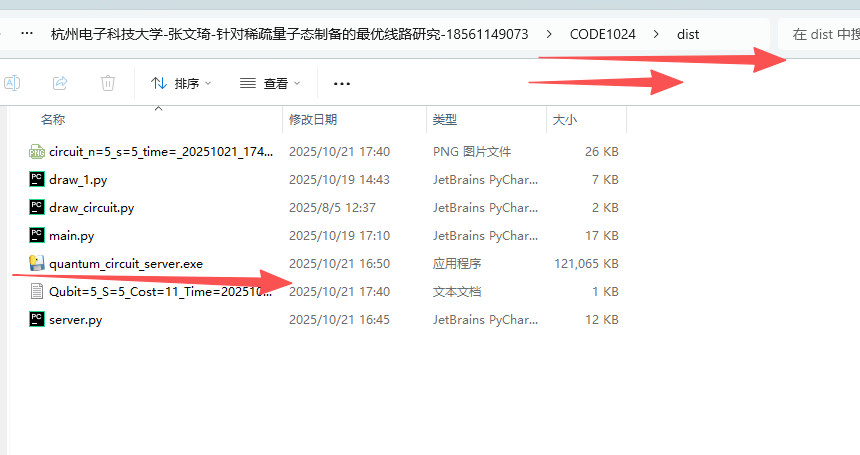
\includegraphics[width=0.55\linewidth]{figure/step1.png}
\end{figure}
2.输入量子比特数量与非零相位数量\par
3.随后选择量子态输入方式：随机生成/手动输入/JSON文件导入\par
4.点击运行算法，程序会检查输入参数的正确性，算法运行完成后会在同目录下生成对应的量子线路图\par
\begin{figure}[H]
    \centering
    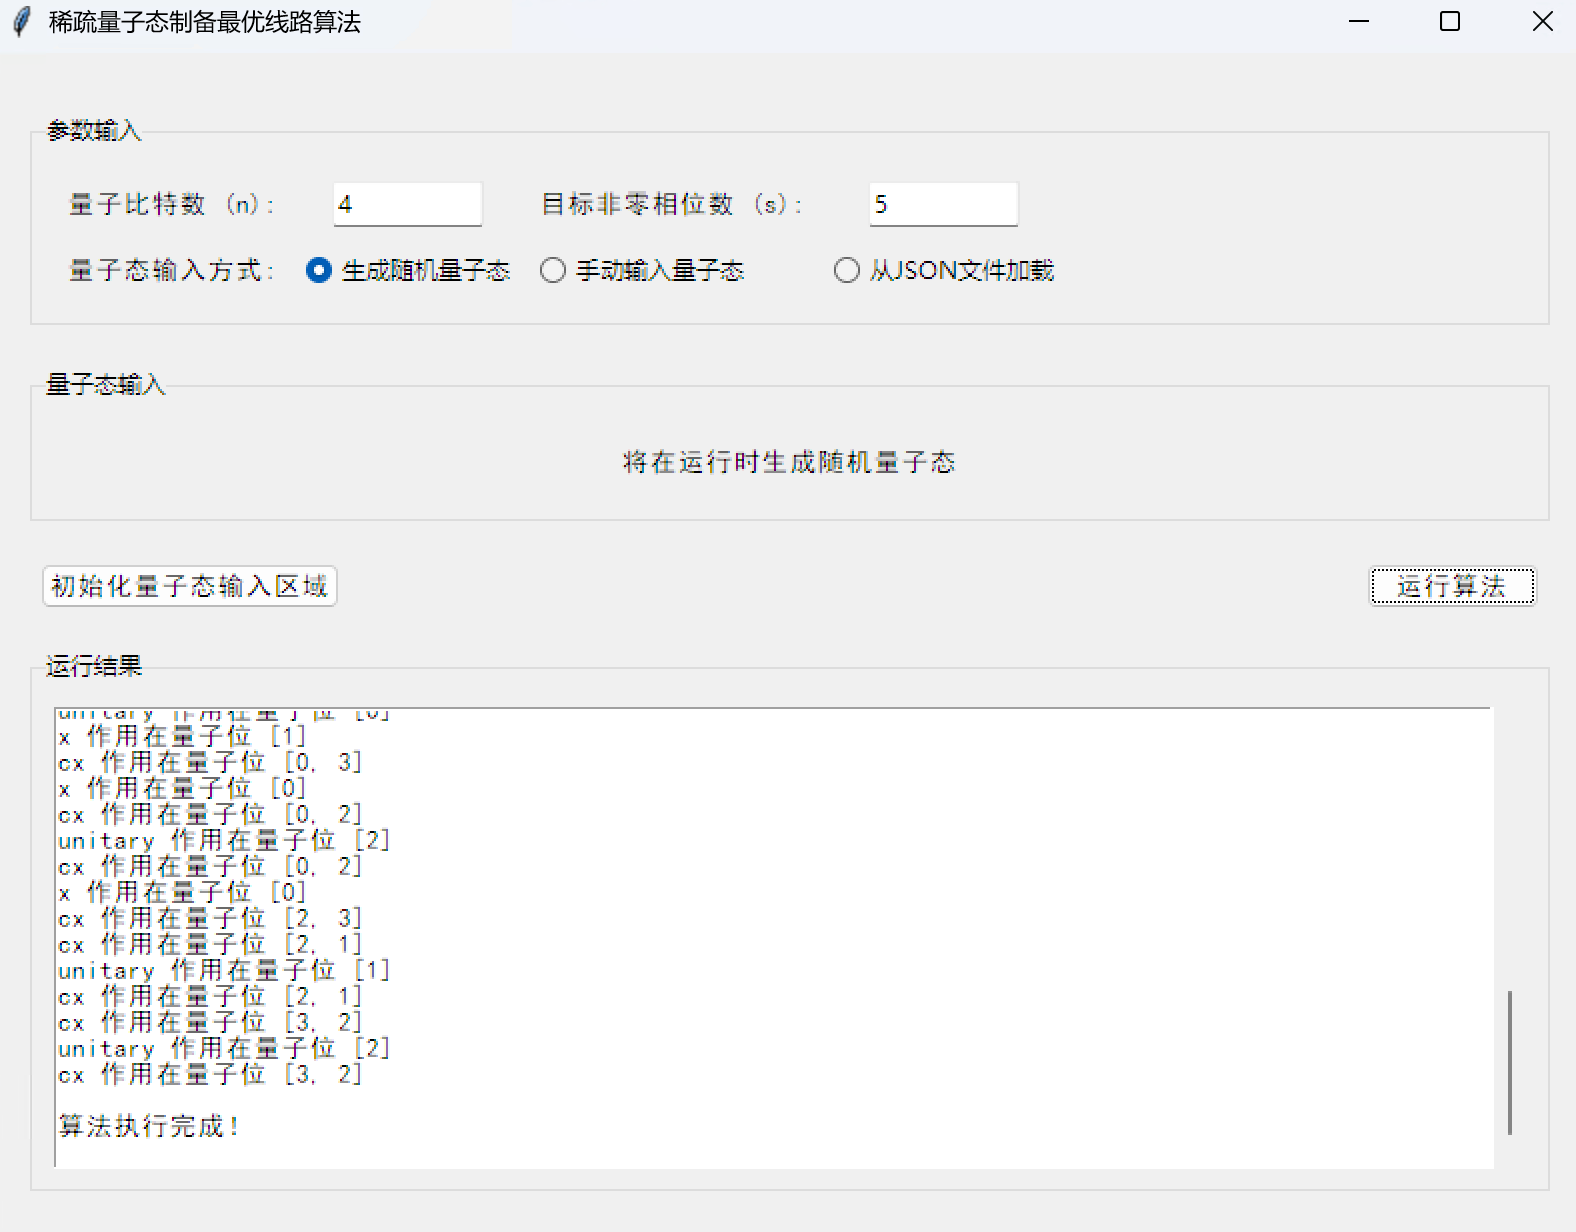
\includegraphics[width=0.55\linewidth]{figure/step2.png}
\end{figure}

\textbf{B.5 性能测试}

为评估算法在不同参数下的平均性能，可运行多轮测试脚本。在项目根目录下执行：python main\_cost\_test.py。该脚本将自动进行多次实验，统计线路开销，输出性能分析结果，适用于算法对比与鲁棒性验证。

\textbf{B.6 线路图展示}

程序运行完成后会在主目录下生成线路图片文件。示例如下

\begin{figure}[H]
    \centering
    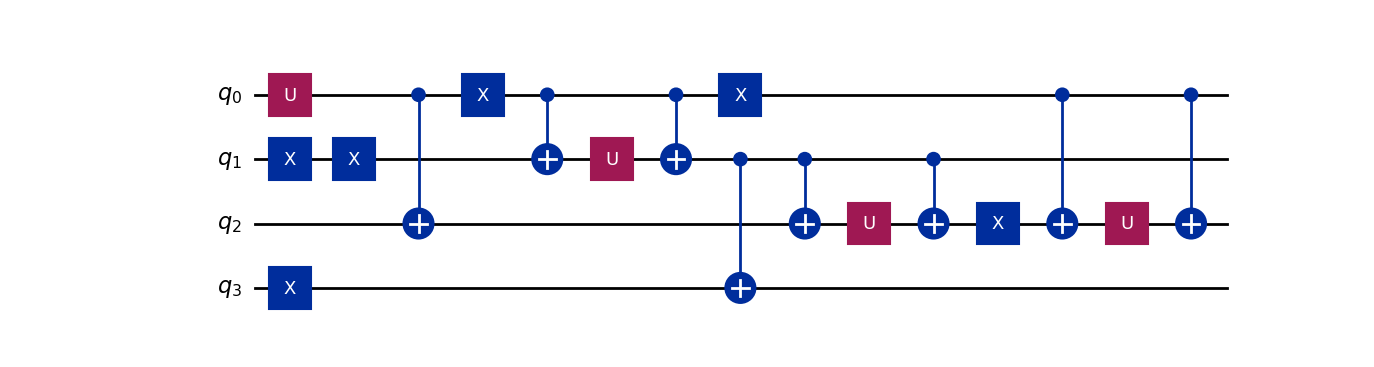
\includegraphics[width=0.8\linewidth]{figure/circuit_n4_s5.png}
    \caption{circuit\_n=4\_s=5}
    \label{fig:circuit_n=4_s=5}
\end{figure}

\textbf{B.7 线路输出格式}\\
程序运行完成后会在主目录下生成线路文字文件，方便用户调用。示例如下：

\begin{verbatim}
x 3
x 1
CCCG 0 []
x 1
cx 2 0
x 0
CCCG 1 [0]
x 0
cx 3 1
CCCG 2 [1]
x 2
CCCG 2 [0]

注：x为not门，格式为[x 作用比特位]
   cx为Cnot门，格式为[x 受控位 控制位]
   CCCG为多控G门，格式为[CCCG 受控位 [多控制位]]


\end{verbatim}

%%%%%%%%%%%%%%%%%%%%%%%%%%%%%%%%%%%
%%%%%%%%%%%%%%%%%%%%%%%%%%%%%%%%%%%5

% \newpage

% \begin{multicols}{1}
% \begin{biography}[yourphotofilename.jpg]
% \noindent
% \textbf{First A. Author}\ \ *第1作者提供照片电子图片，尺寸为1寸。英文作者介绍内容包括：出生年,学位(或目前学历),职称,主要研究领域(\textbf{与中文作者介绍中的研究方向一致}).*
% *字体为小5号Times New Roman*
% \end{biography}

% \begin{biography}[yourphotofilename.jpg]
% \noindent
% \textbf{Second B. Author} *英文作者介绍内容包括：出生年,学位(或目前学历),职称,主要研究领域(\textbf{与中文作者介绍中的研究方向一致})。*
% *字体为小5号Times New Roman*
% \end{biography}
% \end{multicols}


% \begin{multicols}{1}
% \zihao{5}
% \noindent \textbf{Background}

% \zihao{5-}{
% \setlength\parindent{2em}
% *论文背景介绍为\textbf{英文}，字体为小5号Times New Roman体*

% 论文后面为400单词左右的英文背景介绍。介绍的内容包括：

% 本文研究的问题属于哪一个领域的什么问题。该类问题目前国际上解决到什么程度。

% 本文将问题解决到什么程度。

% 课题所属的项目。

% 项目的意义。

% 本研究群体以往在这个方向上的研究成果。

% 本文的成果是解决大课题中的哪一部分，如果涉及863$\backslash
% $973以及其项目、基金、研究计划，注意这些项目的英文名称应书写正确。}

% \end{multicols}

\end{document}


